\chapter{Project Classification} 
\label{chap:3}
\section{Solutions}

\noindent Based on what we discussed about the difficulties in previous section, there's some solutions that came up with multiple cross-chain projects. They will be illustrated in following paragraphs.
\subsection{Ensure the atomic of transactions}
\subsubsection{Atomic swaps}
\noindent An atomic cross-chain swap\cite{herlihy2018atomic} is the basic theoretical framework for multiple parties exchange assets across multiple blockchains. Atomic operations in computer science ensures every exchange either success or failure, no third intermediate state.\\
\noindent For a more intuitive introduction to the atomic swap protocol, we assume an exchange scenario:
   \begin{figure}[H]
    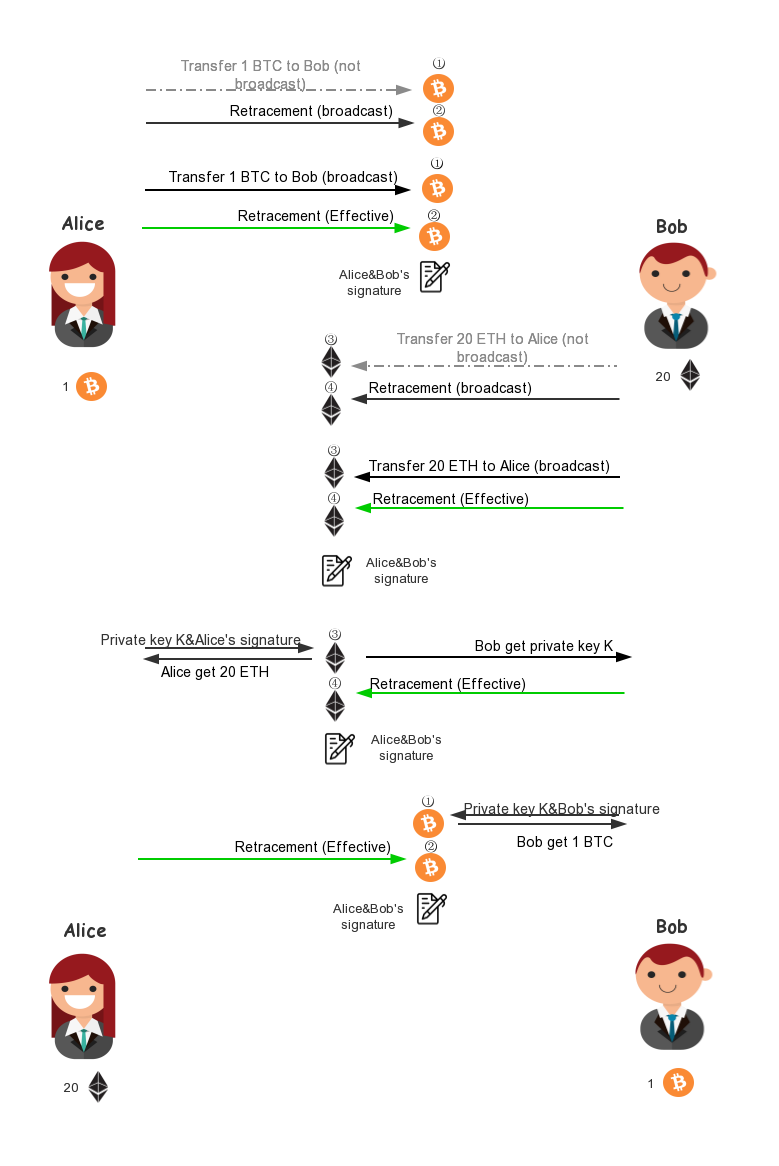
\includegraphics[width=0.79\textwidth]{./figures/atomic_swaps.png}
    \centering
    \caption{Atomic swaps diagram}%\protect\footnotemark}
    \centering
    \label{fig:atomic}
    \end{figure}
\begin{enumerate}
  \item Assume Alice has 1 BTC on chain A while Bob has 20 ETH on chain B, and Alice wants to change Bob's 20 ETH with one BTC. Both Alice and Bob have wallet addresses on both chains A and chain B.
    \item In order to initiate this transaction, Alice needs to randomly generates a key K, which is known only to Alice and then initiates a 1 BTC on chain A transaction (transaction \textcircled{1}) to Bob. The transaction can be only finished when obtains the signature of Bob and provides the key K.
    \item Before broadcast transaction \textcircled{1}, Alice will first broadcast a retracement (transaction \textcircled{2}). If transaction \textcircled{1} does not receive the correct key and signature within 48 hours, the amount paid by that will be returned to Alice. Transaction \textcircled{2} must be signed by Alice and Bob after the broadcast to take effect. At the same time, Alice will only broadcast the transaction \textcircled{1} to the network if transaction \textcircled{2} is successfully validated.
    \item Bob now sees the transaction \textcircled{2} sent by Alice. If Bob agrees, he will sign the transaction \textcircled{2}, of course, Alice will also complete the signature so that the retracement will take effect. Then Alice will broadcast the transaction \textcircled{1} to the whole network.
    \item Bob can only get the value K after he pays Alice with 20 ETH. Hence Bob initiates transaction \textcircled{3} on chain B to pay Alice 20 ETH. These 20 ETH are only available if Alice enters the decrypted key K and attaches Alice's signature. To prevent Alice from denying, Bob also issues a retracement transaction \textcircled{4} that requires Alice and Bob to sign together before the broadcast transaction \textcircled{3}, when Alice does not provide the correct key or the signature within 24 hours. then activate the retracement,20 ETH will be returned to Bob.
    \item After Alice sees the transaction \textcircled{4}, both Alice and Bob need to attach their signature to this transaction to take effect. At this time, Bob will broadcast transaction \textcircled{3} to network.
    \item In order to get 20 ETH, Alice will sign transaction \textcircled{3} with the correct value K. For now, transaction \textcircled{3} succeeds, Alice obtains 20 ETH, and Bob obtains key K.
    \item After Bob gets the key K, he goes back to chain A, enters the key K and his signature, and finally gets 1 BTC from Alice.
\end{enumerate}
\noindent From the diagram, we could obtain that the atomic swap protocol does not transfer the assets of Chain A to Chain B, but only the assets ownership of both chains. The total assets of Chain A and Chain B have not changed, so it can only achieve asset exchange between chains and cannot achieve asset transfer.\\
\noindent This solution not only can be applied to the decentralized ledger system, but also to the centralized ledgers. As long as the two systems provide the functions of retracement, time lock, and key lock.

\subsubsection{Hash Time-Locked Contracts(HTLC)}
\noindent HTLC is a very technical implementation of the atomic swap protocol. It guarantees the atomicity of the transaction through the hash lock and the time lock mechanism. In different systems, whether it is a blockchain system or a centralized ledger system, despite the ways of implementing the lock, the principle behind it is the same, that is, only certain hash conditions or time met, the transaction is allowed to take effect.

        \begin{figure}[H]
        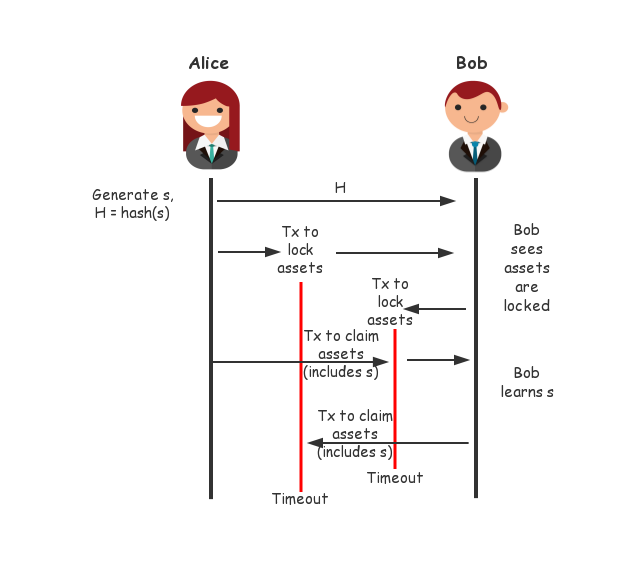
\includegraphics[width=0.8\textwidth]{./figures/Hashlock.png}
        \centering
        \caption{Hash Time-lock Contract diagram}%\protect\footnotemark}
        \centering
        \label{fig:hash}
        \end{figure}
\noindent Using only hash time locks is not enough when you want to achieve cross-chain asset transfer, you also need to cooperate with other cross-chain technologies to ensure the authenticity of cross-chain transactions.
\subsubsection{Hash Time-locked Agreements(HTLA)}
\noindent HTLA is one HTLC generalization protocol came up by Interledger\cite{HTLA}, regardless whether the system support HTLC or not, whether it's a distributed or centralized ledger. HTLA can be used to implement cross-chain exchange between system or even support multi-hop cross-chain interchange between multiple systems, as shown in the Figure \ref{fig:HTLA} below.
   \begin{figure}[H]
    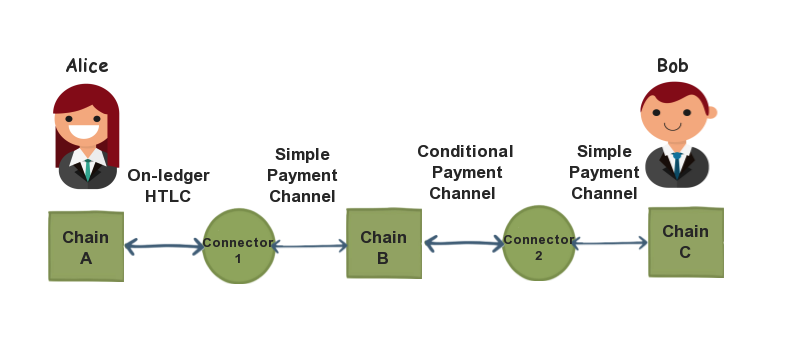
\includegraphics[width=0.8\textwidth]{./figures/HTLA.png}
    \centering
    \caption{Interledger HTLA diagram}%\protect\footnotemark}
    \centering
    \label{fig:HTLA}
    \end{figure}
    
\noindent Alice and Bob can across between blockchains A, B, and C via HTLA, and each blockchain supports different cross-chain protocols. The connector here plays a role in connection and isolation. Linking blockchains that support different cross-chain protocols together, and again isolate them, so that blockchains do not interfere with each other.\\
\noindent HTLA supports multiple cross-chain protocols based on HTLC, some of them are mentioned in Figure \ref{fig:HTLA}.

\subsection{Complete the transaction confirmation}
\noindent As we all know, blockchain systems are relatively independent and closed, there's no direct communication way for them to confirm every piece of records that happened. So no matter how it evolves, there will always be a “middle-man” between the two chains, taking on the role of information exchange between the two chains.\\
\noindent Here the "middle-man" represent any entity that could interact with two chains, it may be one or a group, maybe the centralized or distributed agency, maybe a separate chain or even a functional module. The “middle-man” usually acts as a node for two blockchains at the same time, so that only one application software can be deployed on the same node to obtain the others' system data.\\
\noindent After the “middle-man” completes the data collection, how to confirm the transaction, where to confirm, and who confirms becomes the key point of this problem. According to different schemes, this process can be summarized in three ways:
\begin{itemize}
    \item \textbf{Notary\cite{buterin2016chain}}:\\
    In the notary scheme, a trusted one or group is used to declare to the chain X that an event has occurred on the chain Y, or that the statement is correct. These groups can both automatically or requested to listen and respond to events. There are 3 different child-schemes came up in the evolution of this model: 
    \begin{itemize}
        \item \texttt{Centralized Notary schemes}\\
        The centralized notary mechanism is also called the single-signature notary mechanism, usually played by a single designated independent node or institution, which is the simplest mode. Its purpose is instead of letting Alice and Bob, two strange individuals deal, it's not as reliable as indirect transactions with third-party institutions with credit endorsements (such as Alipay). Since Alice and Bob exist in different ledger systems, the notary is technically required to be compatible with two or more systems at the same time.
        \begin{figure}[H]
        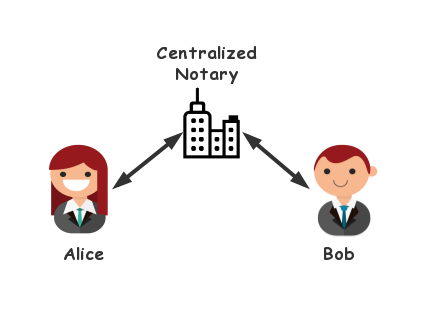
\includegraphics[width=0.7\textwidth]{./figures/cnotary.png}
        \centering
        \caption{Centralized Notary Scheme diagram}%\protect\footnotemark}
        \centering
        \label{fig:cno}
        \end{figure}
        To some extent, the use of centralized institutions has replaced technical credit guarantees, from technical credibility to traditional credit intermediaries. Although this kind of mode has fast transaction processing, strong compatibility, and simple technical architecture, the security of the central node has become a key bottleneck for system stability.
        
        \item \texttt{Multi-sig Notary schemes}\\
       The multi-signature notary mechanism is accomplished by multiple notaries that can sign a common agreement on their respective ledgers to complete the cross-chain transaction. Each node of the multi-signature notary group has its own key, and cross-chain transactions can only be confirmed when a certain number or proportions of notary signatures are reached.

        \begin{figure}[H]
        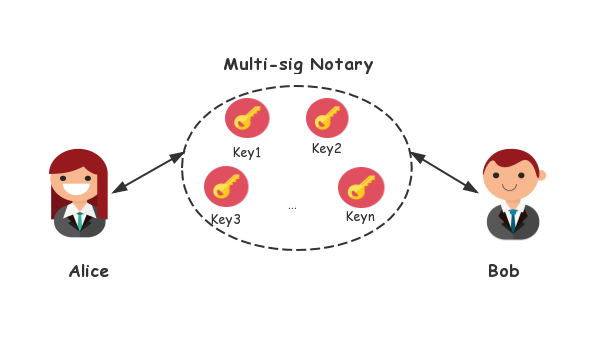
\includegraphics[width=0.8\textwidth]{./figures/mnotary.png}
        \centering
        \caption{Multi-sig Notary Scheme diagram}%\protect\footnotemark}
        \centering
        \label{fig:mno}
        \end{figure}
       This method is more secure than the single-signature mode, and a few notaries who are attacked or do evil will not affect the normal operation of the system. However, this approach requires both chains to have the ability to support multiple signatures.
        \item  \texttt{Distributed signature Notary schemes} \\
        The main difference between distributed signature and multi-signature is the signature generation. Distributed signature using \textit{Multi-Party Computation}(MPC), which will enhance the security as well as the implementation difficulty.
        \begin{figure}[H]
        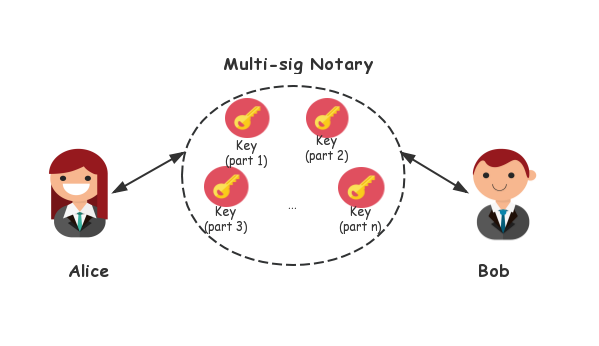
\includegraphics[width=0.8\textwidth]{./figures/dnotary.png}
        \centering
        \caption{Distributed signature Notary Scheme diagram}%\protect\footnotemark}
        \centering
        \label{fig:dno}
        \end{figure}
        As Figure \ref{fig:dno} shows, distributed signature based on cryptography, the key point is that for cross-chain transactions, the system generates one and only one key, and no one in the notary group will have a complete key. The key is randomly sent to each notary node in the form of fragments.
        Meanwhile, the fragment is the processed ciphertext, so even if all the notaries put together the pieces, the complete key cannot be known, and the security of the key is fully guaranteed.
    \end{itemize}
    \item \textbf{Relay\cite{buterin2016chain}}:\\
    Relay is one flexible and easy-to-expand cross-chain technology that does not rely on trusted third parties to help with transaction verification. Instead, it is self-verified by the receiving chain after receiving the send chain data. Self-verification methods are depending on the system structure. For example, BTC-relay\cite{btc-relay} based on \textit{Simplified Payment Verification}(SPV), and Cosmos\cite{cosmos} rely on verify the number of nodes' signature.\\
    \textsc{Vitalik} mentioned Relay in his Chain Interoperability paper\cite{buterin2016chain}, pointing out that chain A and chain B can use the other party's block data for information synchronization and cross-chain calls. Currently, information synchronization can be done, but there is no mature technical solution for cross-chain calls. Two chains cannot verify the validity of each others block at the same time, otherwise, they will fall into an infinite loop of nesting. If chain A owns the block data of chain B, then chain A needs to be confirmed in the case of chain B transaction confirmation, and chain B needs to wait for chain A's transaction confirmation because it also has block A's block data, it goes on as a loop.
    
    
    
    \item \textbf{Sidechains}:\\
     The concept of a sidechain as defined in white paper\cite{back2014enabling} is: \textit{sidechain is a blockchain that validates data from other blockchains}. However, this explanation was considered to be too broad and not rigorous by \textsc{Vitalik Buterin} in \textsc{Chain Interoperability}\cite{buterin2016chain}. "Sidechain” is more frequently used to refer to what Blockstream calls a “pegged sidechain”, where the functionality of a blockchain is of an anchored asset of another asset, which chain is regarded as the parent chain. In this way, this relationship is based on assets, not the blockchain itself. This is a strong coupling cross-chain structure using directly embeds part of the data of the original chain into its own block or storage space. In the case of cross-chain transactions,  verification can be completed directly through the original chain data stored in the system. This method is generally considered bidirectionally at the beginning of the system design.\\
     Compared to notary and relay, the sidechain is more direct. The state of one chain will be directly reflected in the data of the other chain. When one chain is attacked, the other chain may also be affected. This model is more suitable for the design of the same system, which allows the two sides to become a whole without losing the relative independence of the ledgers.

\end{itemize}
\subsection{Realize multiple chains interoperability}
\noindent The computer network connects the original independent computers into a local area network, the local area network develops into a metropolitan area network, the metropolitan area network evolves into the Internet, and the Internet connects the people of the world like never before.\\
\noindent However, for the emerging technology/industry of blockchain, it is still in the “single-machine” era, and the interactions demand between chains and chains will become increasingly strong with the application of blockchain.\\
\noindent To realize interoperability among multiple chains, there are two potential aspects of difficulties that need to overcome: 
\begin{itemize}
    \item How to achieve interoperability among blockchains system that has already developed.
    \item How to prepare/setup the way for the interconnections among the new blockchains in the future.
\end{itemize}

\subsubsection{Active compatibility}
\noindent This solution is mainly aimed at the existing blockchain system. First, there are different blockchain application systems in the upper layer, and then the underlying cross-chain mechanism is developed.\\
\noindent Usually these systems are heterogeneous chains and need to be docked one by one, but there is also a different solution for a pair of connections.
\begin{enumerate}
    \item Direct interconnection between the two chains
        \begin{figure}[H]
        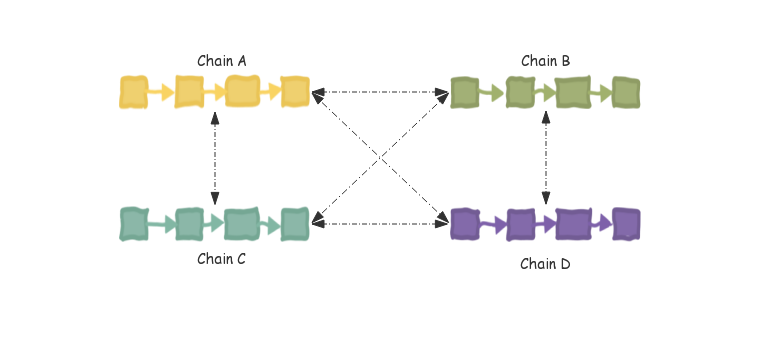
\includegraphics[width=1\textwidth]{./figures/direct.png}
        \centering
        \caption{Direct interconnection network architecture diagram}
        \centering
        \label{fig:direct}
        
        \end{figure}
    This method is the most time-consuming and laborious without the support of the unified underlying protocol. It is necessary to establish 6 paths between the 4 chains to realize the interconnection between them. And each path needs to be customized. Although this method is not scalable, it can guarantee better security and independence. Once an attack occurs, it is difficult to affect the entire network.
    \item Third-party cross-chain platform
      \begin{figure}[H]
        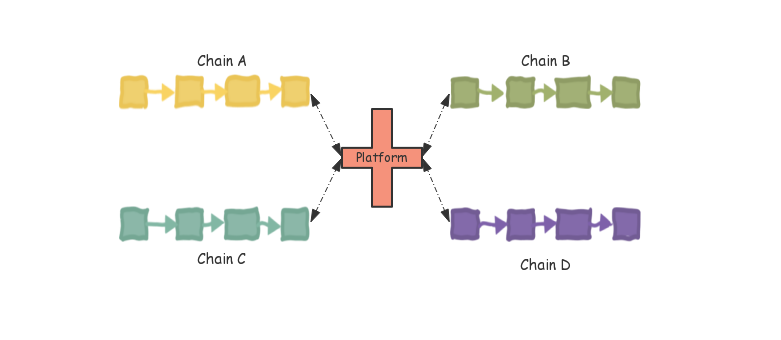
\includegraphics[width=1\textwidth]{./figures/platform.png}
        \centering
        \caption{Cross-chain platform network architecture diagram}
        \centering
        \label{fig:platform}
        
        \end{figure}
    To establish a cross-chain platform, blockchains can indirectly interconnect with each other. Thus, only 4 paths are required to build a cross-chain network. However, in this method, the cross-chain platform will become the key point and performance bottleneck of the entire cross-chain network (not necessarily the bottleneck, but it may be in the future). Once the cross-chain platform is attacked, the entire cross-chain network will be paralyzed.
\end{enumerate}
\subsubsection{Passive compatibility}
\noindent Passive compatibility is mainly aimed at the blockchain system that has not been developed. It first builds the underlying cross-chain platform, allowing other blockchain systems to be easily, conveniently and securely accessed. Cross-chain platforms will prioritize the development of systems and protocol standards that apply to interoperability between the various chains. The subsequent development of standards-compliant development on existing platforms allows for the creation of blockchains that naturally have cross-chain functionality within the system. However, the cross-chain mentioned here refers to the chain that conforms to the protocol standard can be easily connected to each other. If it is to interoperate with other chains outside the system, it is necessary to develop a separate middleware to communicate.\\
\noindent In addition, different cross-chain platforms can support different types of blockchains, such as Cosmos supporting isomorphic chains and Polkadot supporting heterogeneous chains, both of which are highly scalable, and will be later discussed in Section \ref{sec:p}.

\section{Project study}
\label{sec:ps}

\subsection{Lightning Network}
\noindent In general, we can not say lighting network realize the cross-chain function, though it provided a typical application towards atomic swaps and HTLC. The design idea of the lightning network is straightforward. It put a large number of high-frequency small-value transactions off-chain to expand the transaction processing capability of the blockchain.\\
\noindent Lightning network\cite{poon2016bitcoin} is a fast and scalable Bitcoin transaction project, and it has two main technical points:
\begin{enumerate}[A.]
    \item \textbf{Recoverable Sequence Maturity Contract} 
    
    	RSMC is similar to a reserve mechanism in which both parties trade in an
    	off-chain trading pool.  This trading pool is a ``micro-payment channel''.
    	When a transaction occurs between two parties, the proportion share of the
    	common assets in the trading pool will change. The new proportional data
    	needs to be signed and confirmed by both parties, and the old proportional
    	share version is invalid. The entire process is completed off the chain,
    	so it does not occupy the resources of the main chain. The final
    	proportion of assets will be confirmed, and record to the main-chain after
    	one of the transaction party requires a withdraw.
    	
    	It could happen anytime as long as both parties signed for this. To ensure
    	the security, if someone submitted the old share of assets to make
    	profits, others could protect themselves by proving this balance sheet is
    	not the latest one. Then the asset of the counterfeit party will be
    	confiscated to the challenger.
    \item \textbf{Hash Time-locked Contract}
    
     Lightning Network uses HTLC to guarantee the atomicity of transaction, as
     shown in Figure \ref{fig:hash}. 
     
     This diagram illustrates how HTLC works to
     provide limited-time transfer function. The basic process is: Bob and Alice
     can reach an agreement that specifies Alice to lock a certain amount of
     assets and provide a hashed value of $H$. Before the arrival of time $T$, if
     Bob can learn an appropriate $s$ (secret) where it's hash value matches with
     $H$ and sent to Alice, Bob can get the corresponding amount of assets value.
     Conversely, the asset will unlock and return to Alice.
\end{enumerate}
\noindent When there are ``micro-payment channels'' between multiple users, these channels are connected to form a ``channel network'', which is the lightning network. The mutual transfer of the two parties does not require a direct payment channel to connect with, through the intermediary can also achieve mutual transfer. \\ \\
\noindent \begin{large}
\textbf{Disadvantages}:
\end{large}
\begin{itemize}
    \item Users cannot pay off-line. 
    \item More suitable for small transactions. Large transfer amount needs to open multiple channels.
    \item Easy to face the dis-matched situation, if there's no response from one party, the other one may need hours to close the channel and substitute with another route.
\end{itemize}


\subsection{Notary Scheme}
\label{sec:notary}
\subsubsection{Ripple Interledger protocol}
\noindent Earlier we focused on cross-chain, this project is more focused on cross-ledger, which means that the agreement not only supports decentralized blockchains but also supports various centralized ledgers, which is broader support for cross-chain applications. Ripple ILP\cite{thomas2015protocol} uses the HTLA and Notary scheme to implement this technology.\\
\noindent Ripple is the first project to propose the use of blockchain technology to achieve cross-ledger exchange of assets, with a focus on resolving cross-border remittances, enabling faster and more economical international remittances via the Ripple network.\\
\noindent Interledger Protocol(ILP) is compatible with any online ledger systems. Specifically, the ILP will establish a two-way pegged relationship between the trader's account and a Ripple local account, enabling simultaneous changes between the two to ensure transparency in the transaction process. At the same time, for two ledger systems that do not have a direct payment channel, multi-hop indirect cross-ledger transactions can be realized through ILP. \\
\noindent The main idea of ILP is to secure cross-ledger transactions by setting up \textit{escrow account} on Ripple. So the process will need the preparation of escrow account of several parties in the transaction. As an example in Figure \ref{fig:ILP}, Alice, Bob, and one selected market maker should have their own Ripple escrow accounts set up on two bank systems before the transaction. \\
\begin{itemize}
    \item Alice first selects a market maker with the most suitable exchange rate, and fill in the remittance information, receipt address and timeout period on the Ripple application.
    \item This information will be packed by the Interledger Module and sent to the Ripple Account 1, Ripple Account 1 records the changed amount of currency in the escrow account 1 and sends the transfer certificate to the \textbf{Validator}
    \item For Bob, Company B fills in the Ripple application with information such as the remittance address and timeout period and broadcasts it on the Ripple network. At this time, the liquidity provider selected by A will transfer a certain amount of assets in B's currency from Ripple Acc.3 to Ripple Acc.2 in advance, then send the transfer certificate to the \textbf{Validator}
    \item Validator checks the two transfer certificates; after the verification is passed, the ILP ledger will be liquidated simultaneously according to the Hashed Time Lock Agreement.
    \item The final step is when liquidation completed, Ripple will synchronize all account changes through an interledger module, thus realizing the cross-ledger transactions.
\end{itemize}
        \begin{figure}[H]
        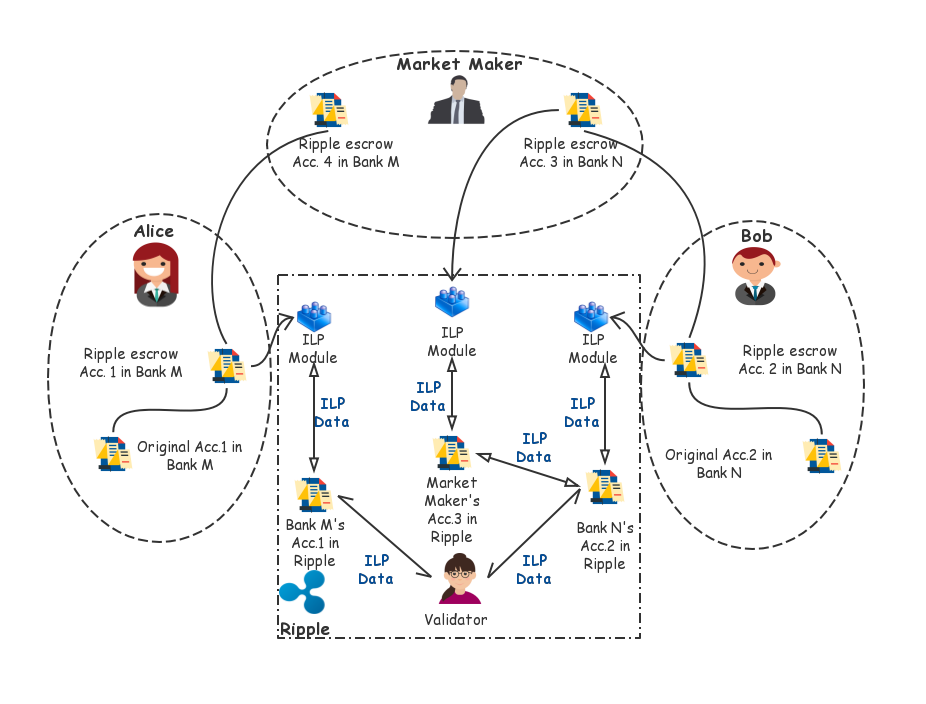
\includegraphics[width=1\textwidth]{./figures/ILP.png}
        \centering
        \caption{ILP example process}%\protect\footnotemark}
        \centering
        \label{fig:ILP}
        \end{figure}
\subsubsection{Wanchain}
\noindent Wanchain\cite{wanchain.org} is a cross-chain platform project initiated in 2016. It is a heterogeneous cross-chain framework that implements cross-chaining based primarily on distributed notary scheme. This model mainly uses cryptography "Secure Multi-Party Computation" and "Threshold Key Sharing Scheme" to implement the Authenticator's distributed signature.\\
\noindent Wanchain provides the infrastructure for asset cross-chain transfer channels for different blockchain networks, realizing the transfer of assets between Wanchain and original chain. Wanchain3.0 now launches bridges from Bitcoin to the Ethereum network. The transaction reliability verification is completed by multiple Storeman of Wanchain. The following figures\ref{fig:wan1}\ref{fig:wan2} are shown the transfer process between Wanchain and Ethereum.
        \begin{figure}[H]
        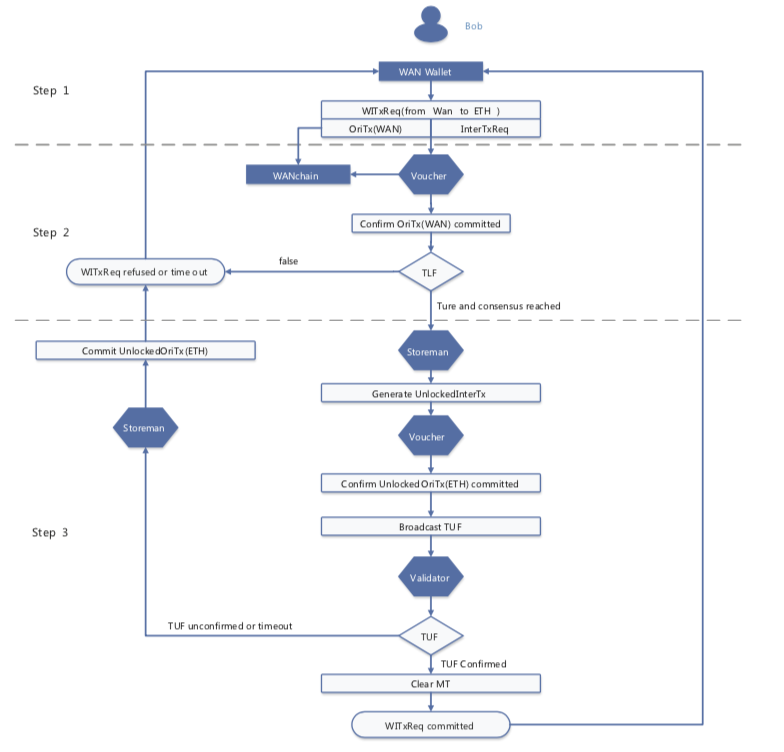
\includegraphics[width=1\textwidth]{./figures/ethtowan.png}
        \centering
        \caption{{Data transfer process from Ethereum to Wanchain}\protect\footnotemark}
        \centering
        \label{fig:wan1}
        
        \end{figure}
\footnotetext{Image courtesy of Wanchain white paper\cite{wanchain.org}}
        \begin{figure}[H]
        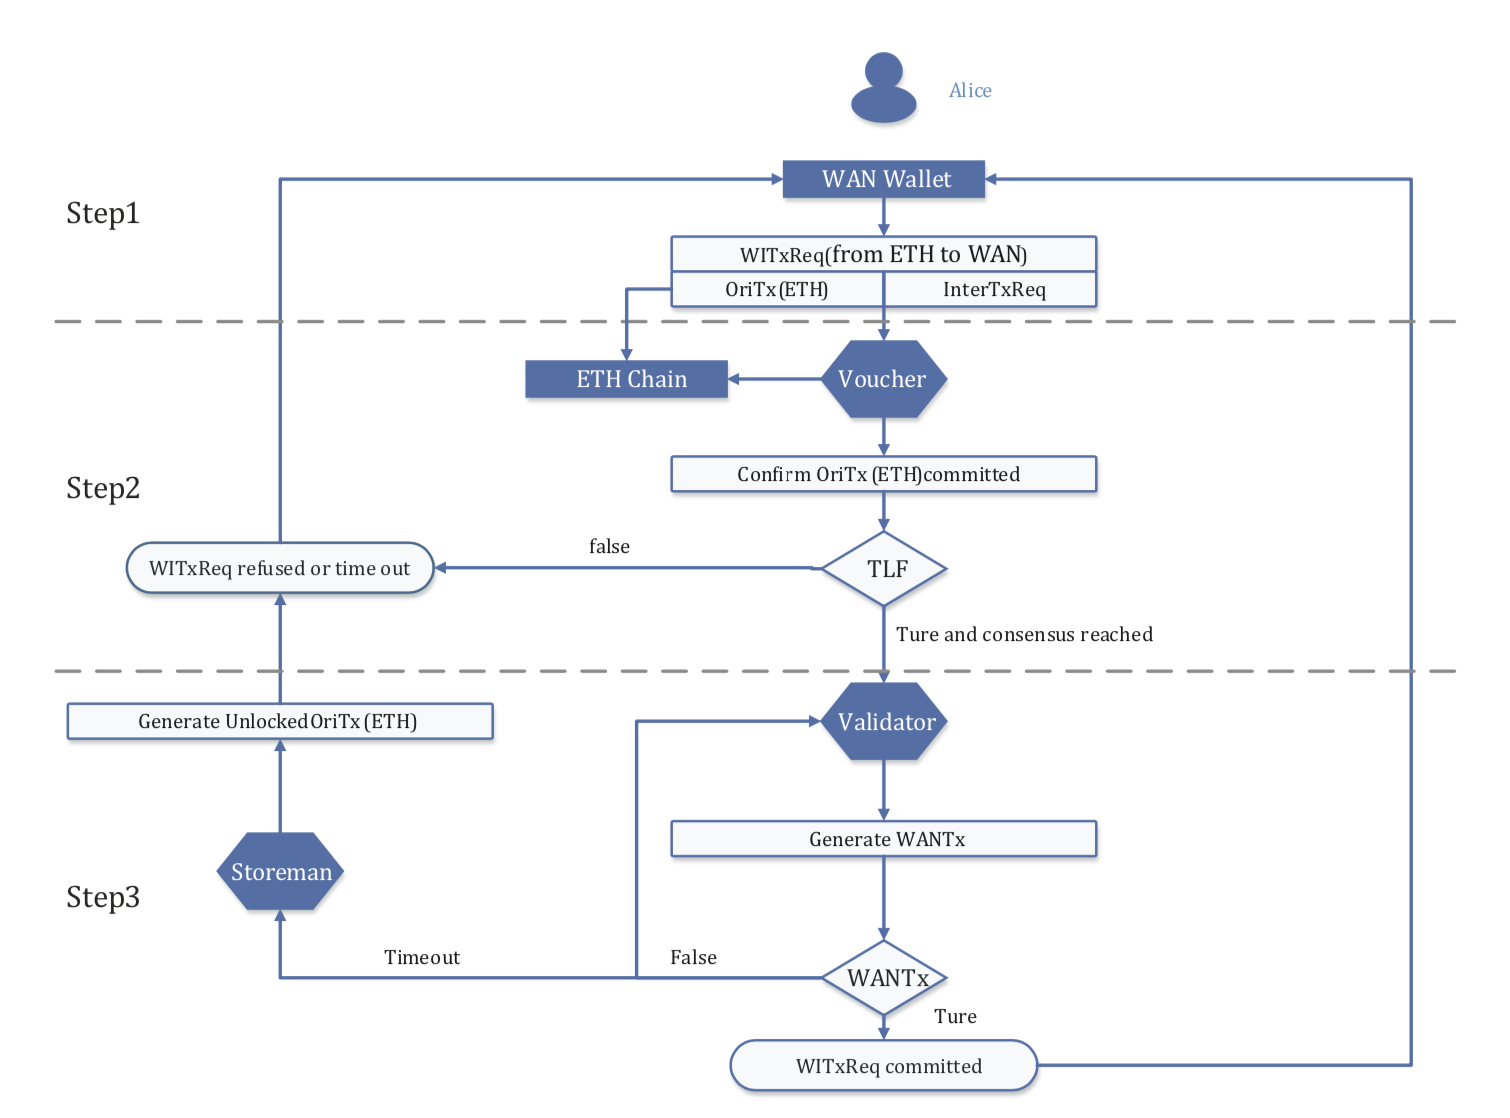
\includegraphics[width=1\textwidth]{./figures/wantoeth.png}
        \centering
        \caption{{Data transfer process from Wanchain to Ethereum}\protect\footnotemark}
        \centering
        \label{fig:wan2}
        
        \end{figure}
\footnotetext{Image courtesy of Wanchain white paper\cite{wanchain.org}}

\begin{enumerate}
    \item The token of the user in the original chain will be sent to Wanchain in the locked account, and the transaction is locked by Hash Time Lock;
    \item After the \textbf{Voucher} verified  the transaction on the original chain, the \textbf{Storeman} will initiate a cross-chain contract transaction on the Wanchain, and transfer the mapping token in wanchain to the user's cross-chain account on Wanchain, and locked;
    \item After the user's wallet detects the transaction locked by the cross-chain contract, release the Secret to the cross-chain contract;
    \item Storeman obtains the control of the original chain token through the secret number, thus achieving confirmation of the original chain transaction.
    \item If the user does not release the secret number within the scope of the hash time lock, the hash time lock expires
    \item The transaction of the post-cross-contract is automatically invalidated, and the user regains control of the original token.
\end{enumerate}
\noindent In Wanchain, when Storeman locked an account, the private key of the locked account is scattered into multiple pieces and send to Storeman, and it requires more than a certain percentage of Storeman complete the signature before the final confirmation. In order to avoid conspiracy, Storeman has to pay a certain amount of token to participate in the verification in case of doing evil. To ensure atomicity, Wanchain uses a hash time lock to lock cross-chain transactions, ensuring that no user or Storeman will complete a one-sided transaction.\\
\noindent Since the Wanchain mechanism does not change the original chain, it is necessary to adapt the development according to the characteristics of the original chain, which is also the difficulty of heterogeneous cross-chain solution. The transaction speed is affected by the confirmation speed of the original chain.\\\\
\begin{large}
\textbf{Fusion}
\end{large}\cite{fusion}\\


\noindent Similar to the principle of Wanchain, Fusion's goal is to build a basic platform for the operation of encrypted financial applications based on blockchain technology. On this platform, a variety of tokens can be freely interacted through smart contracts to achieve value interoperability. Support multi-platform cross-chain asset transfer, using a distributed signature notary model for cross-chain transaction processing.\\
\noindent Based on Hierarchical Hybrid Consensus Mechanism(HHCM), Fusion combines the advantages of PoW and PoS consensus mechanism, which balancing the safety, efficiency, and scalability. It is the only cross-chain platform that offers parallel computing, multiple triggering mechanisms, and off-chain data support.\\

        \begin{figure}[H]
        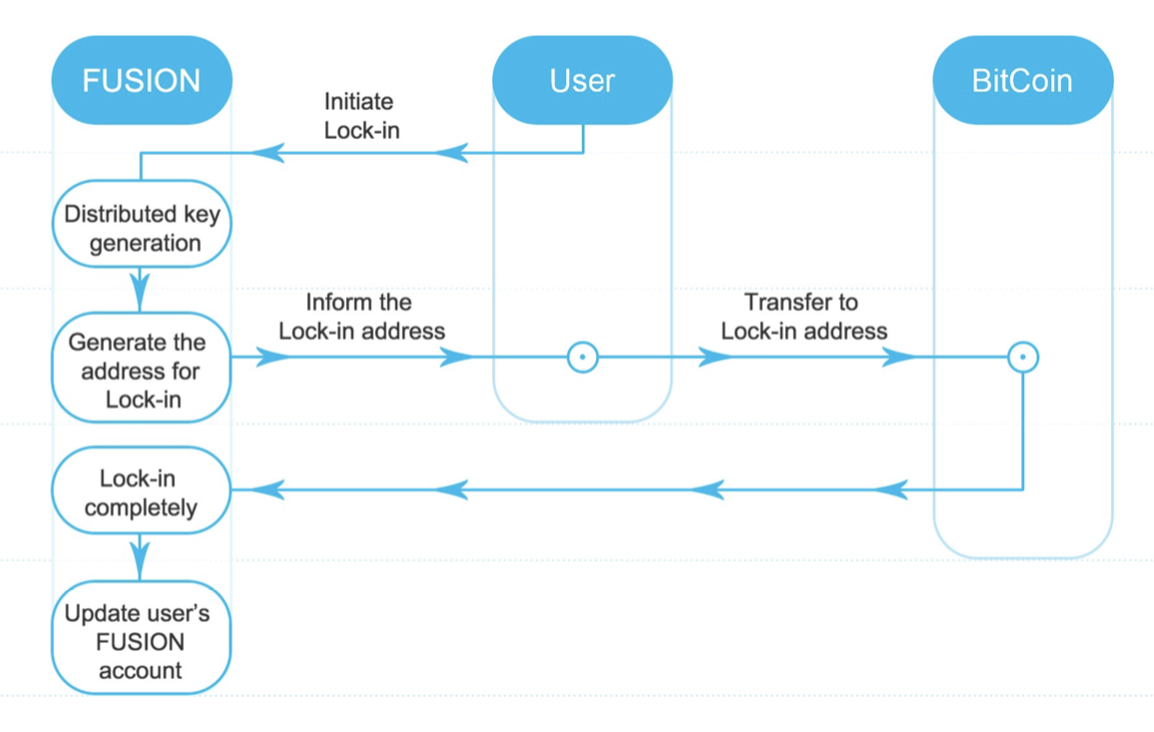
\includegraphics[width=1\textwidth]{./figures/lockin}
        \centering
        \caption{{Fusion Network Architecture, lock-in process}\protect\footnotemark}
        \centering
        \label{fig:lockin}
        
        \end{figure}
\footnotetext{Image courtesy of Fusion white paper\cite{fusion}}
\noindent The realization of cross-chain assets transaction is based on the lock-in\&lock-out process as shown in Figure \ref{fig:lockin}.

\subsection{Relay Scheme}
\subsubsection{BTC-Relay}
\noindent In 2016, the BTC-Relay released by the Consensys team is the most classic relay cross-chain solution, enabling cross-chain transactions between Ethereum and Bitcoin, as well as realizing Ethereum's DApp applications to support BTC payments. Since Bitcoin scripts are non-turing complete and difficult to support complex applications, BTC-Relay only implements one-way cross-chain from Bitcoin to Ethereum.
        \begin{figure}[H]
        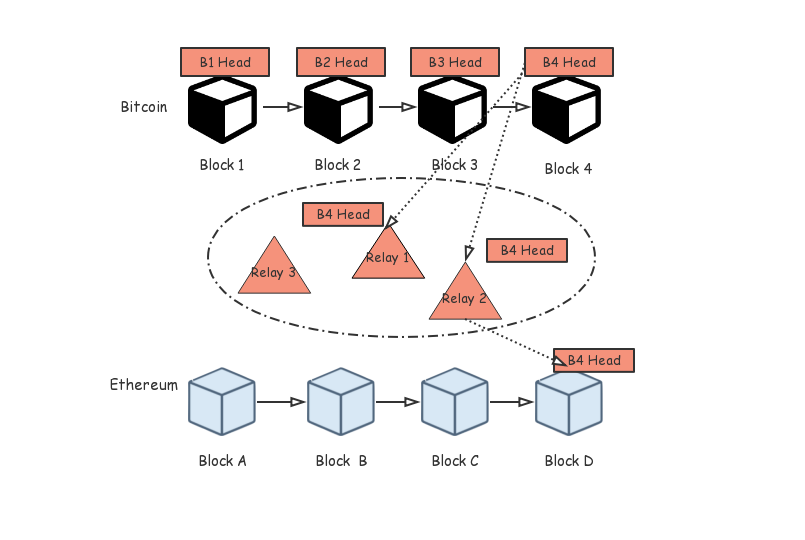
\includegraphics[width=1\textwidth]{./figures/btc.png}
        \centering
        \caption{BTC-Relay cross-chain process diagram}%\protect\footnotemark}
        \centering
        \label{fig:btc}
        \end{figure}
\noindent Like Figure \ref{fig:btc} shows, BTC-relay itself is a smart contract for Ethereum. The function of the contract is to verify certain transactions on Bitcoin and provide verification information to other DApp users on the Ethereum. Relay is a group of users who obtain block header data from Bitcoin and has the account address of the Ethereum network. The Relay that submits the block header data to the BTC-Relay contract as soon as possible can get the ETF transaction fee reward. After obtaining the block header data, the BTC-Relay smart contract can verify a transaction according to the principle of SPV proof. When a transaction in the Bitcoin network does occur, it can trigger the specific transaction or smart contract execution of the Ethereum network.

\subsubsection{Cosmos}
\noindent Cosmos\cite{cosmos} is a cross-chain platform project initiated by the Tendermint team in 2017. It supports the modular establishment of Cosmos isomorphism chain and also supports the external heterogeneous chain through Bridge. Its most important feature is that all the chains in the Cosmos system are isomorphic chains and can more easily support the flow of assets across the chain. All the zones share a set of network protocols, consensus mechanisms, and data storage methods. Assemble the new Zone blockchain through the API interface.\\
\noindent The overall architecture of Cosmos network are shown in Figure\ref{fig:cosmos}:
        \begin{figure}[H]
        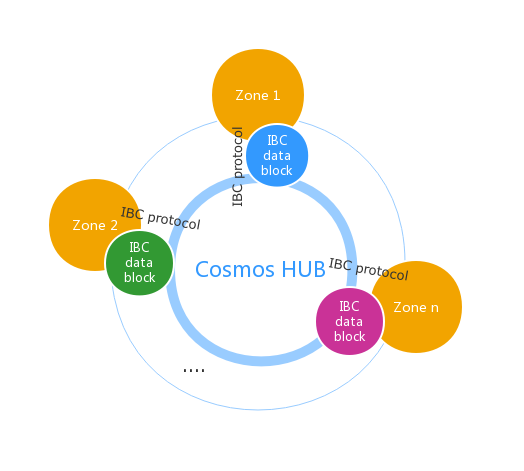
\includegraphics[width=0.7\textwidth]{./figures/cosmos.png}
        \centering
        \caption{Cosmos network architecture}%\protect\footnotemark}
        \centering
        \label{fig:cosmos}
        \end{figure}
        
\noindent There are many Zones connected to the Hub (Hub is a chain, and each Zone is also a chain). Cosmos Hub maintains a multi-asset distributed ledger and masters the asset status of all the Zones that connected to it. Each zone will synchronize the status of the Hub, but the communication between the Zone and the Zone can only be done indirectly through the Hub. Each cross-chain asset transfer requires a common confirmation of the zone, hub, and receiving zone to be successful. 
\par The information is transmitted between zones through packets based on the IBC (Inter-Blockchain Communication) protocol. The blocks in a space pack the data to be delivered into standard IBC data packets and finally complete the transmission through the network layer UDP or TCP protocol.
        \begin{figure}[H]
        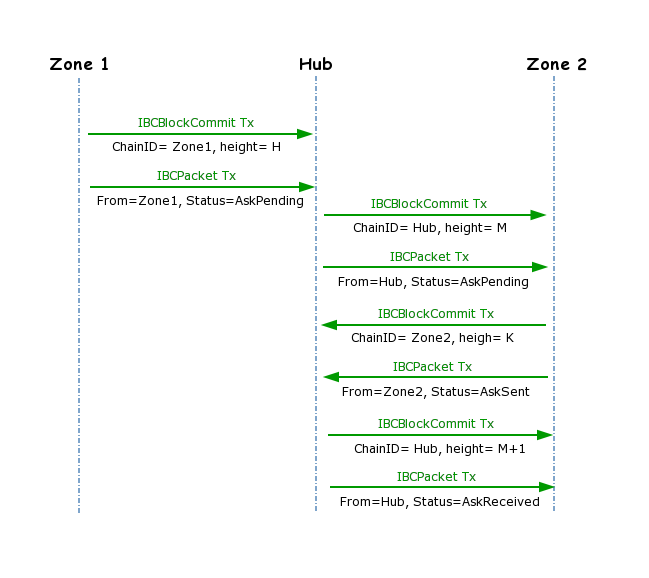
\includegraphics[width=0.8\textwidth]{./figures/IBC.png}
        \centering
        \caption{IBC sequence diagram}%\protect\footnotemark}
        \centering
        \label{fig:IBC}
        \end{figure}
\begin{enumerate}
    \item  Zone 1 initiates an IBCBlockCommitTx transaction, passing the new block header information (including all Validator's public key) to the HUB;
    \item  Zone 1 initiates an assets transaction;
    \item Zone 1 verifies the transaction;
    \item Send the valid transaction into the message queue for HUB;
    \item Zone 1 listens to a new message in the queue, which generates Merkle proof, and sent to HUB as IBCPacketTx's Payload. (In each space there is an independent third-party relay program that generates Merkle Proof from the original chain and assembles it into a Packet and initiates the transaction, passing it to the receiving chain);
    \item HUB verifies that Merkle Proof is valid, if it is valid, send a message to Zone2 (The process of sending a message to Zone2 by HUB is the same as steps 1~6);
    \item Zone2 verifies that Zone1 is a valid transaction after receiving the HUB message. Send a message to HUB confirming that it can receive assets from Zone1;
    \item The HUB sends a message to Zone2, sends the asset to Zone 2, and the asset transaction is completed.
\noindent Due to an attack or network error during the transfer process, it is possible for the message sent by Zone 2 to the HUB is lost, as shown in the figure\ref{fig:timeout} below, after waiting for a period of time, the HUB sends a message telling Zone1 that the current transaction is timeout and the transaction fails.
\end{enumerate}
        \begin{figure}[H]
        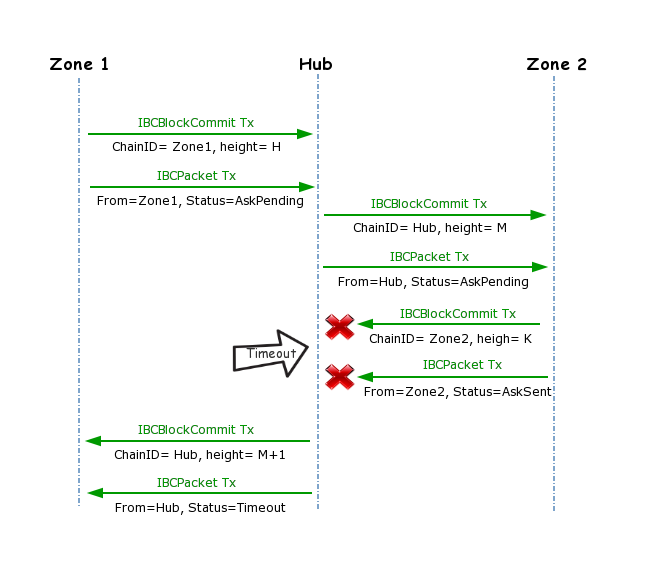
\includegraphics[width=1\textwidth]{./figures/IBC_timeout.png}
        \centering
        \caption{IBC sequence diagram, timeout}%\protect\footnotemark}
        \centering
        \label{fig:timeout}
        \end{figure}
        
\noindent Cosmos based on \textbf{Tendermint} consensus which is the combination of PBFT and PoS, it improves the processing power of Cosmos Network. The cross-chain transaction between Cosmos and other heterogeneous blockchains need to be carried out through Cosmos Bridge, Bridge-Zone will be responsible for the docking with the original chain, including the confirmation of the original chain transaction, create or destroy the corresponding tokens.\\
\noindent Overall, Cosmos is a blockchain development framework, allowing developers to focus on their own business without having to consider the underlying technology of the blockchain so the plug-in design can use Cosmos as needed.


\subsubsection{Polkadot}
\noindent Polkadot\cite{polkadot} is a cross-chain project supported by the Web3 Foundation. Creating a scalable, heterogeneous, multi-chain architecture designed to address blockchain interoperability, scalability, and security.\\
\noindent The overall architecture of Polkadot is shown in the figure below, consisting of a Relay Chain, Parachains and Bridges. 
\begin{itemize}
    \item \textbf{Relay chain} is the central system of the Polkadot network, which coordinates the consensus and transactions between the chains, records account information and transaction status; 
    \item \textbf{Parachains} can be built by developers to collect and process transactions, and transfer to Relay chain;
    \item \textbf{Bridges} connect other heterogeneous blockchains (such as Ethereum) with Polkadot network.
\end{itemize} 
\noindent There are four roles in Polkadot's network:
\begin{enumerate}
    \item Collators (collecting user transactions, validating and submitting to Validators),
    \item Validators (validating and broadcasting transaction data committed by Collators, verifying blocks and paying deposits)
    \item Nominators (investment deposits selected for trust Validators)
    \item Fishermen (supervising the evil behavior in the network). 
\end{enumerate}
\noindent Collators and Validators are the performers of the main transaction when doing cross-chain operations, while Nominators and Fishermen are the participants in maintaining system trust.\\


\begin{figure}[H]
    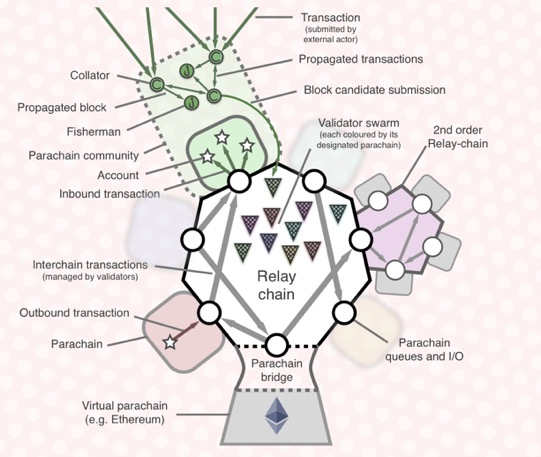
\includegraphics[width=1\textwidth]{./figures/Polkadot.jpg}
    \centering
    \caption{Polkadot network architecture \protect\footnotemark}
    \centering
\end{figure}
\footnotetext{Image courtesy of Polkadot white paper\cite{polkadot}}

\noindent Parachain can share trust of the entire Polkadot network, but it also gives a certain confirmation right to the Relay chain; when the user's transaction information on Parachain A is transmitted to Parachain B, the process is as follows:
\begin{enumerate}
    \item The initiated transaction is sent to the Collator on Parachain A;
    \item Collator validates the transaction and packs it into the block; 
    \item Collator submits the block and state transition proof to the Validator on Parachain A;
    \item The Validator verifies the block it receives that contains only valid transactions and pays a certain amount of deposit;
    \item  After enough Nominators have paid a deposit for the Validator, they broadcast the block to the Relay Chain;
    \item The transaction of data has been executed.
\end{enumerate}
\noindent Unlike Cosmos, Polkadot supports cross-chain interoperability between heterogeneous chains. It does not only support asset transactions, but also the data transfer. Its system complexity and implementation are more difficult than Cosmos.

\subsubsection{ICON}
\noindent ICON\cite{icon} is committed to building a cross-chain network that connects all types of blockchain systems, enabling DApps to be interconnected across all types of blockchains. The cross-chain transactions primarily handled through notary mechanism. Figure \ref{fig:concept} below shows the overall conceptual model of ICON. With ICON, blockchains are connected around the \textbf{Nexus}, which is a loopchain-based blockchain. The whole system based on loop fault tolerant mechanism which is an enhancement of BFT-based algorithm.  \\


 \begin{figure}[H]
        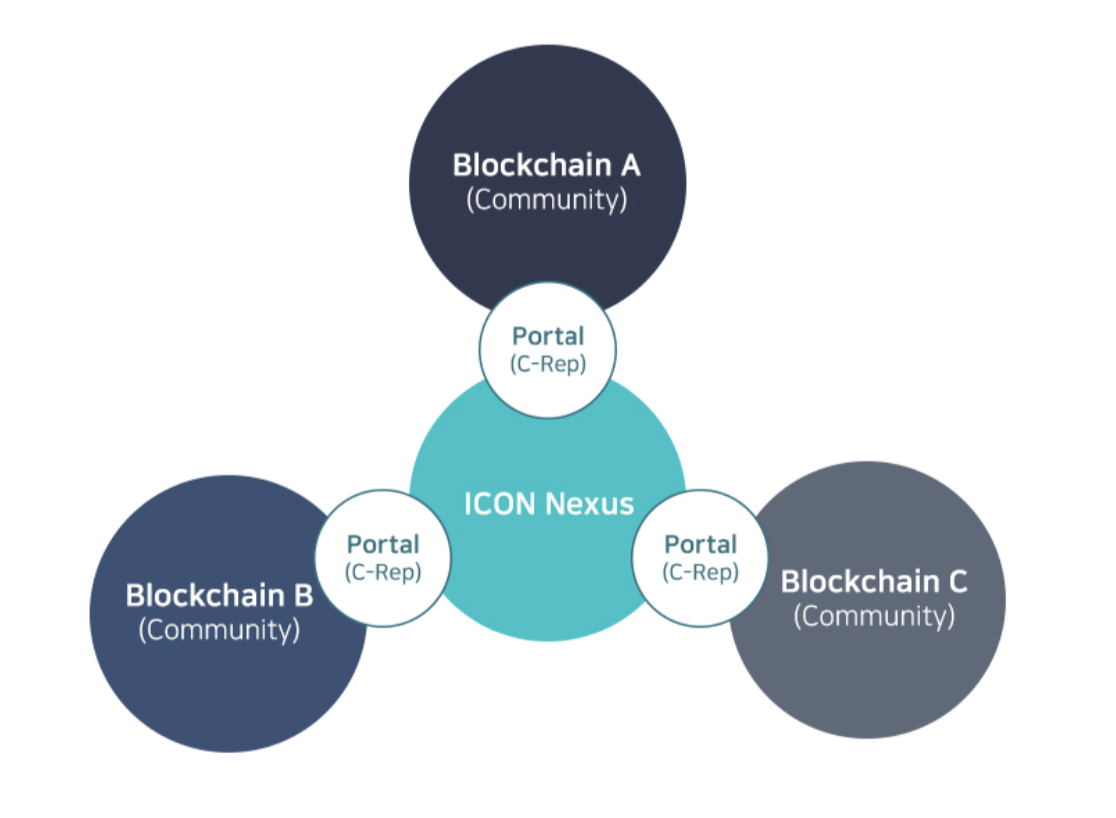
\includegraphics[width=1\textwidth]{./figures/iconconcept.png}
        \centering
        \caption{{Conceptual model of ICON}\protect\footnotemark}
        \centering
        \label{fig:concept}
        
        \end{figure}
\footnotetext{Image courtesy of ICON white paper\cite{icon}, Nexus is a Multi-Channel blockchain comprised of Light Client of respective blockchains. Each blockchain connected to Nexus via a portal.}
        \begin{figure}[H]
        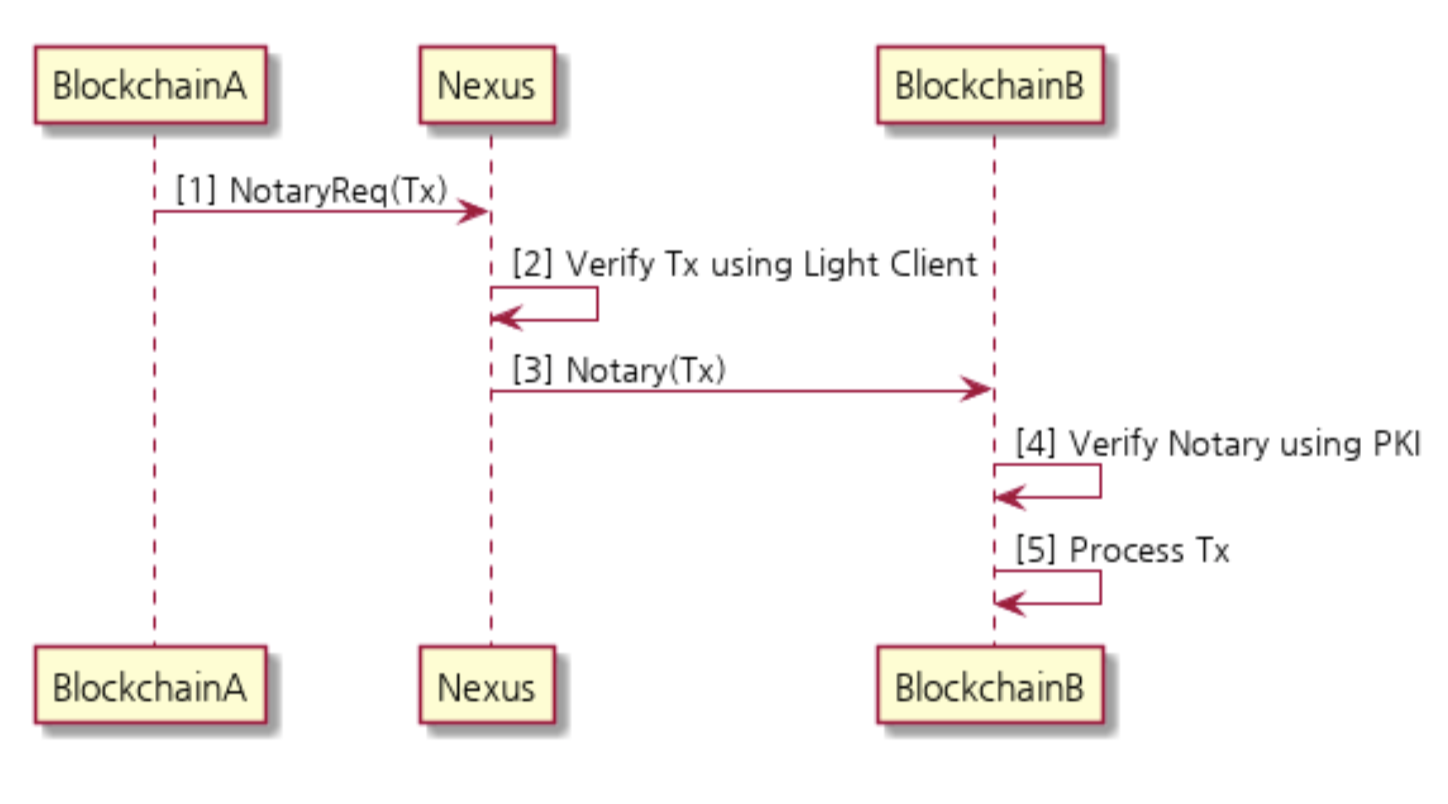
\includegraphics[width=1\textwidth]{./figures/icontrans.png}
        \centering
        \caption{{Assets transaction process through Nexus}\protect\footnotemark}
        \centering
        \label{fig:icon}
        
        \end{figure}
\footnotetext{Image courtesy of ICON white paper\cite{icon}}
\noindent Although rated as one slow progress cross-chain project, ICON still has the ambition to not only connect blockchains together but also aiming at realizing communication between the traditional ledger system and the blockchain world.


\subsubsection{AION}
\noindent Among the Interoperability Alliance\protect\footnotemark
 \footnotetext{Wanchain, ICON and AION form an alliance to overcome the technical difficulties towards cross-chain technology. reference: https://medium.com/helloiconworld/blockchain-interoperability-alliance-icon-x-aion-x-wanchain-8aeaafb3ebdd}
, AION differs from Wanchain and ICON. While the other two projects still focus on the assets and value transactions cross-chain, AION also expanding the business logic and interoperability between chains. Figure\ref{fig:aion} represents a simple multi-tier network architecture based on AION.
        \begin{figure}[H]
        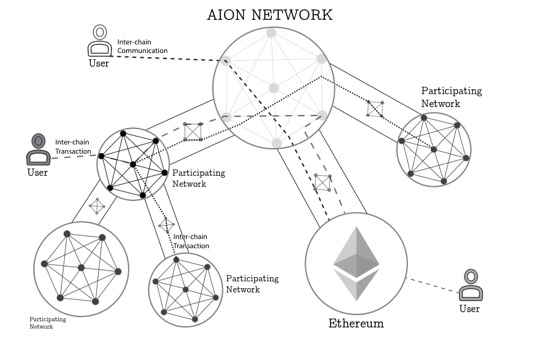
\includegraphics[width=1\textwidth]{./figures/aion.jpg}
        \centering
        \caption{{Multi-tier network structure of AION}\protect\footnotemark}
        \centering
        \label{fig:aion}
        
        \end{figure}
\footnotetext{Image courtesy of AION white paper\cite{aion}}
\noindent AION aims to establish a multi-tier cross-chain platform that supports interoperability of heterogeneous chains. By connecting networks and bridges to blockchain systems, the route of cross-chain transactions is a multi-stage process. \\
\noindent At each stage, the Validators verifies the transaction and agrees on whether the transaction is forwarded or rejected. Bridge validators will use a lightweight BFT-based algorithm to reach consensus. If a transaction is rejected at any time, any state changes due to cross-chain transactions will be revoked, at least in the connected network.\\
\noindent AION has different consensus mechanisms at different product stages, the latest AION 3.0 using mixed DPoS and PoI algorithm.\\
\noindent AION is an emerging project and still in the early stage of development.

\subsubsection{Quant Overledger}
\noindent Developed by Quant Network, Overledger is the one Blockchain Operating System that facilitates the development of multi-chain smart contracts\cite{verdian2018quant}. In order to not limit the inter-communication between 2 blockchains at the same time, Overledger enables reading the transactional, contract and script information and map them into one ``over layer''. And in most cases where the transaction requires multiple hops during the route to the destination, Overledger will create a common interface among ledgers to solve this issue.\\
\noindent Different from other projects who devote their cross-chain solution into the transactional layer,




\subsection{Sidechain Scheme}
\label{sec:side}


\subsubsection{Plasma}
\noindent As the second-layer expansion framework of Ethereum, Plasma has been proposed by \textsc{Joseph Poon} (founder of Lightning Network) and \textsc{Vitalik Buterin} (founder of Ethereum) in 2017 \cite{poon2017plasma}. The first thing to be clear is that Plasma is essentially a set of frameworks instead of a separate project. It provides an off-chain solution for a variety of different project real projects. \\
\noindent Layer 2 expansion of blockchains often known as off-chain expansion, similar to lightning network, this kind of expansion scheme does not need to modify the underlying protocol of the blockchain, but by transferring a large amount of frequent calculation work "off-chain", and submitting the calculation results to the "main chain" guarantee its finality as we discussed previously. Plasma works like blockchains in blockchains where anyone can create different Plasma on top of the underlying blockchain to support different business needs. \\
\noindent As an example of sidechain, Plasma derived from the general concept of symmetric 2-way pegged scheme to realize the transfer solution. The overall process of asset exchange is shown in figure \ref{fig:2way}. 
        \begin{figure}[H]
        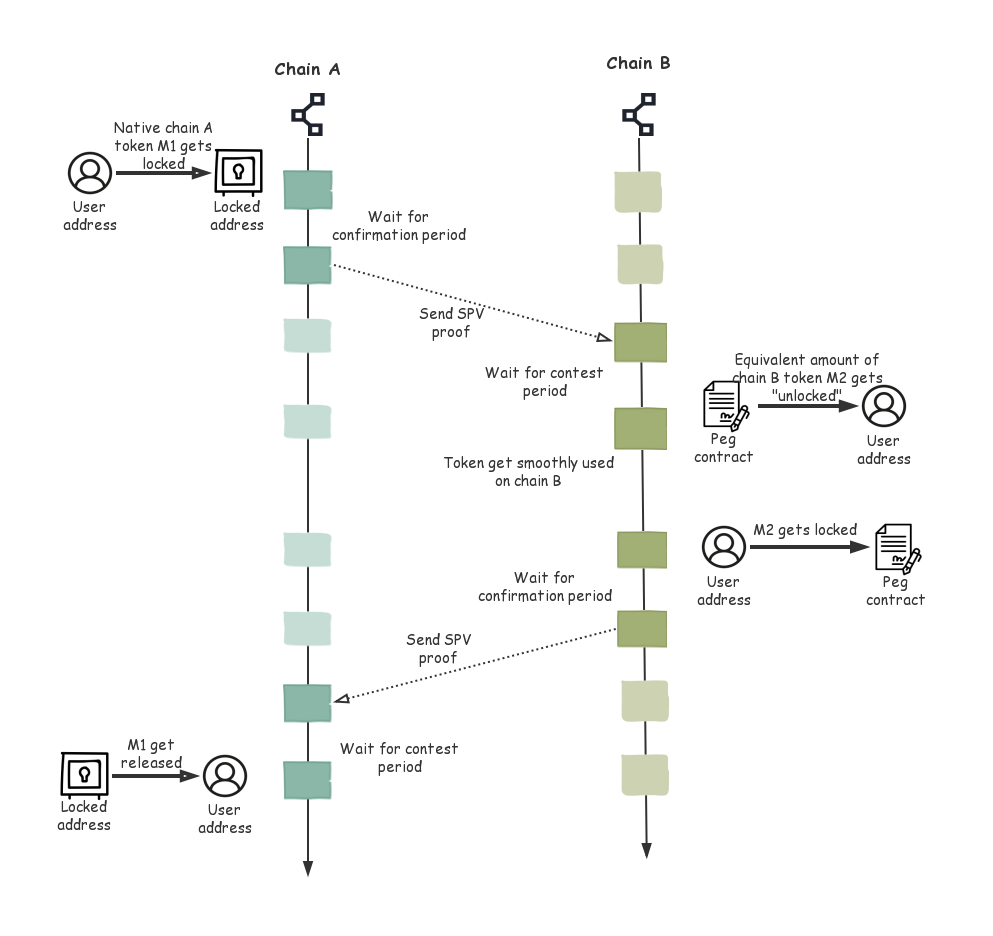
\includegraphics[width=1\textwidth]{./figures/2way.png}
        \centering
        \caption{{2-way pegged sidechain diagram}\protect\footnotemark}
        \centering
        \label{fig:2way}
        
        \end{figure}
\footnotetext{SPV to verify that the transaction exists (recognized by other nodes on the blockchain)}
\begin{enumerate}
    \item When chain A wants to transfer the asset to chain B, it first needs to initiate a transfer transaction Tx1 (chain A's locking addr1 + chain B's receiving address addr2), and the asset M1 is locked on the addr1.
    \item After Tx1 transaction is submitted, it is necessary to wait for a \textit{confirmation period} so that there are enough blocks and calculations to ensure that the cross-chain transaction Tx1 is confirmed, reducing the impact of refactoring on cross-chain transactions.
    \item After the confirmation period, the \textbf{SPV} certificate containing Tx1 will be sent to chain B. B knows that chain A has indeed initiated and locked asset M1, so it generates a corresponding amount of M2 on chain B according to a certain ratio. The value of M1 is transferred to M2 means the assets on chain A are transferred to chain B.
    \item After M2 is generated on B, it is necessary to wait for the \textit{competition period} before unlocking M2 to avoid double-spend attack in chain A reconstruction.
    \item After unlocking, M2 can freely circulation on chain B.
    \item The process of a transaction from chain B to chain A is similar to previous steps.
\end{enumerate}
\noindent Plasma supports multi-level sidechains and uses MapReduce mode to perform parallel computing, which greatly improves sidechain performance. The block header and hash data of the side chain will be sent to the main chain, and \textit{Proof of Fraud} can be used to ensure the correctness of the sidechain transaction.


\subsubsection{Liquid}
\noindent Liquid\cite{Liquid} is a sidechain of BTC and a typical representative of the multi-signature notary mechanism. It is designed to meet the BTC fast transfer needs of exchanges, market makers and brokers. Therefore, Liquid uses the multi-sig federation mechanism to confirm the transaction block, which can greatly improve the transaction speed.\\
\noindent Liquid based on Element codebase and uses Strong Federation technology to support 1:1 Bitcoin exchange. The basic process of the transaction is described as Figure \ref{fig:multisig}. The confirmation of this asset transfer requires multi-signature from the majority of notaries.

        \begin{figure}[H]
        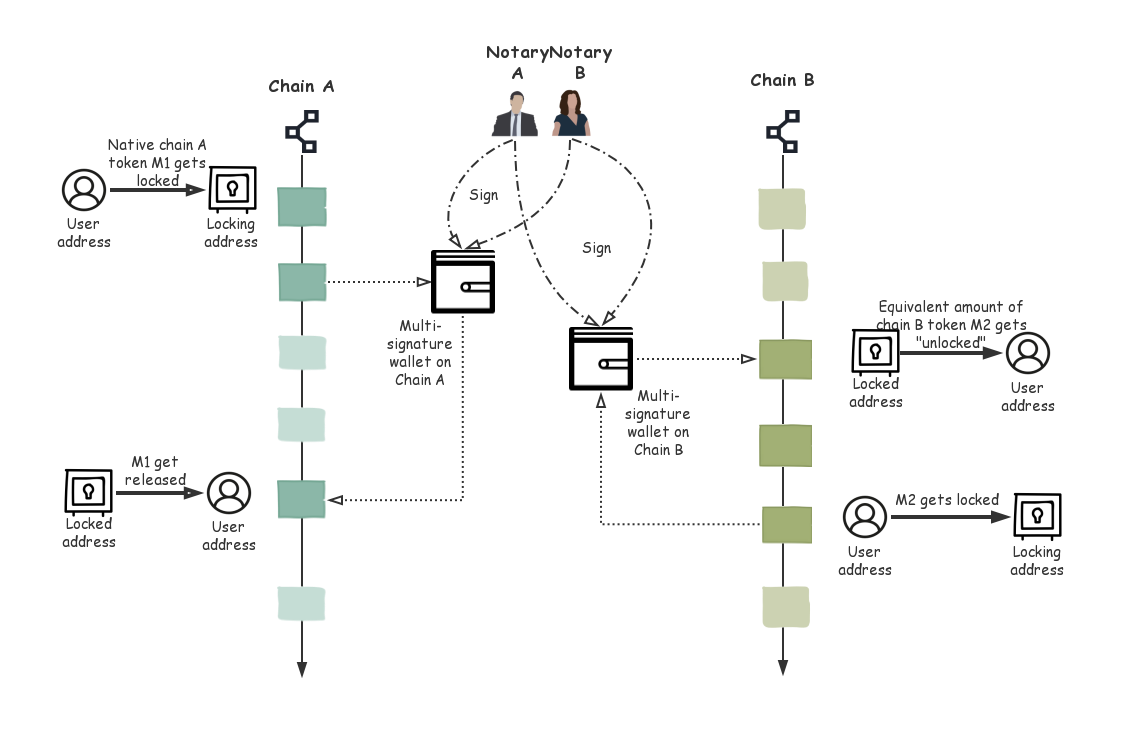
\includegraphics[width=1\textwidth]{./figures/multi_sig.png}
        \centering
        \caption{Multi-signature federation scheme}%\protect\footnotemark}
        \centering
        \label{fig:multisig}
        \end{figure}
        
\noindent In Strong Federation, there are 2 types of node role in the network:
\begin{itemize}
    \item Blocksigners: Signature verification for transactions in the sidechain to achieve block consensus. 
    \item Watchmen: When the asset is transferred from the sidechain to the main chain, it is responsible for signature verification of the transaction on the main chain, indicating that the sidechain asset has indeed been destroyed, and the main chain can unlock the corresponding number of assets.
\end{itemize}

\subsubsection{Elastos}
\noindent In order to ease the pressure on the main chain as well as provide better user experience for DApps, Elastos\cite{Elastos} adopted the main chain + sidechain architecture,  main chain only responsible for the circulation of the ELA while the DApps run on the sidechain. \\
\noindent In this scenario, the transfer of the assets between the main chain to sidechain is in a one-to-many relationship. It is feasible that the side chain only saves all the block header information of the main chain. If the main chain needs to save the block header information of all the side chains, it will lead to poor scalability. So Elastos uses asymmetric 2-way peg scheme based on SPV to realize the cross-chain function.\\
\noindent Assets from the main chain to the sidechain, Elastos using SPV proof to prove the transactions, while it secures the transfer using multi-signature notary scheme when transfer from sidechain to the main chain. We can regard this process as a combination of Plasma and Liquid.

\subsubsection{OneLedger}
\noindent As one cross-chain consensus protocol, OneLedger\cite{Oneledger} uses sharding and improved practical Byzantine fault-tolerant consensus. By creating sidechain, it can easily realize cross-chain interactions between individuals or business in OneLedger. OneLedger defines a three-layer consensus protocol to integrate different blockchain applications more efficiently.\\
\noindent Different from what we have discussed before, OneLedger as a sidechain, it realizes the synchronization of assets and values between the main chain and sidechain by applying multi-sig federation and drive-chain.\\
\noindent A drivechain\cite{lerner2016drivechains} gives custody of the locked coins to the miners, allowing them to (algorithmically) vote on when to unlock coins and where to send them. As Figure \ref{fig:drive} shows:
        \begin{figure}[H]
        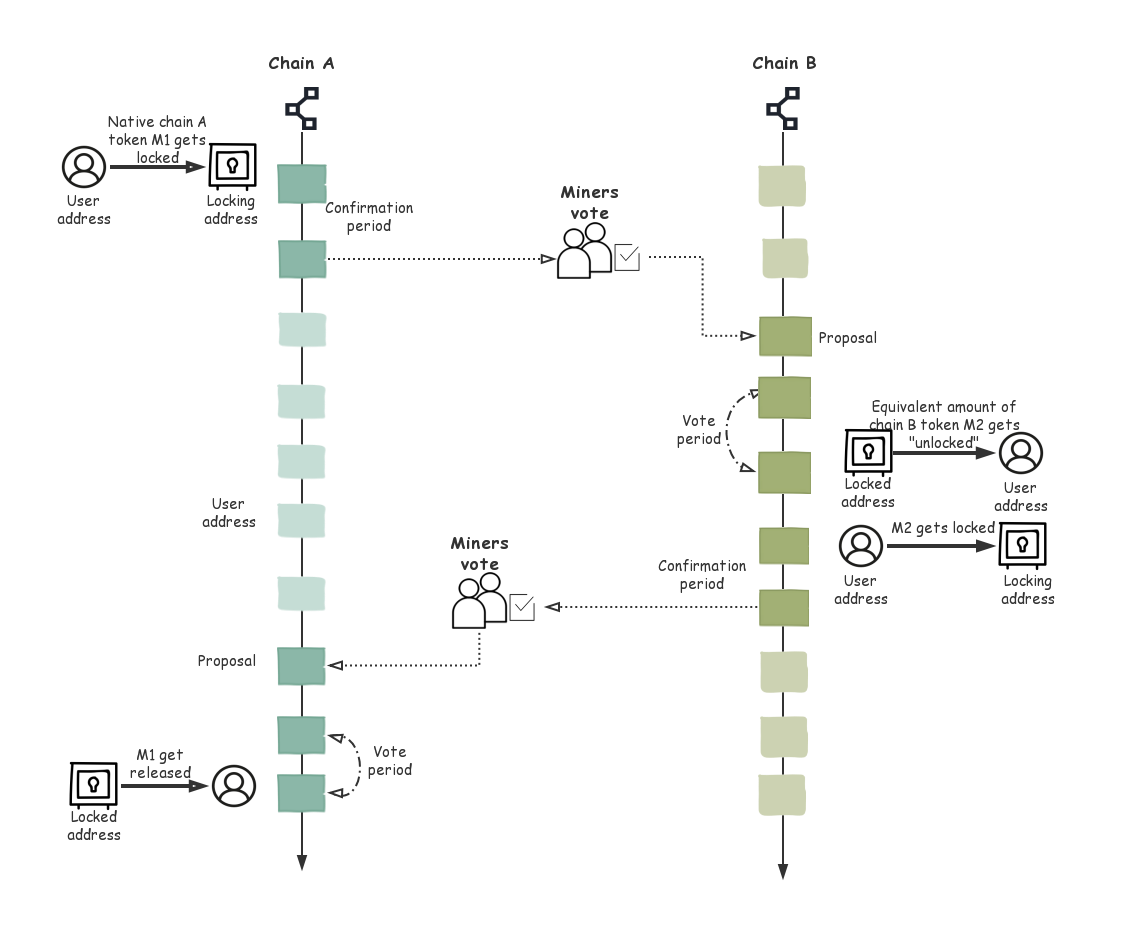
\includegraphics[width=1\textwidth]{./figures/drive.png}
        \centering
        \caption{Drivechain  working diagram}%\protect\footnotemark}
        \centering
        \label{fig:drive}
        \end{figure}
\noindent According to OneLedger's white paper, the core of OneLedger is a set of consensus protocols that enable OneLedger to effectively integrate different blockchain products. As far as I understand that the protocol mentioned here is not a specific consensus protocol algorithm in the traditional sense, but a series of concepts and application scenarios. Among all 3 layers, I specifically studied the \textit{Public Chain Consensus} which apply on the atomic transfer between blockchains through OneLedger Network on the base layer.
        \begin{figure}[H]
        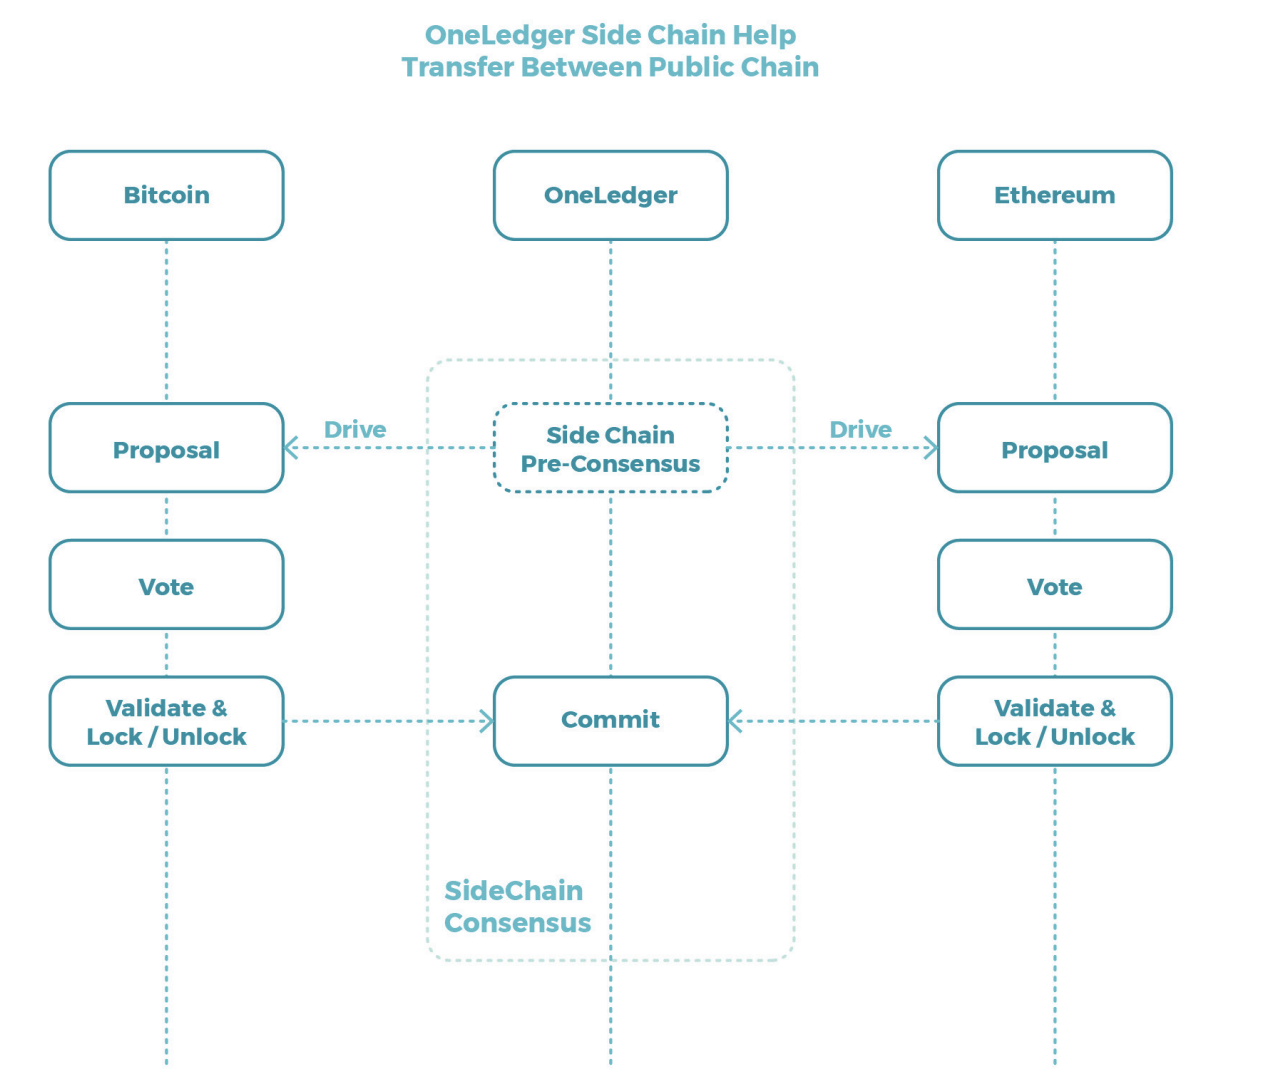
\includegraphics[width=1\textwidth]{./figures/oneledger.png}
        \centering
        \caption{{OneLedger sidechain architecture}\protect\footnotemark}
        \centering
        \label{fig:oneledger}
        
        \end{figure}
\footnotetext{Image courtesy of OneLedger white paper\cite{Oneledger}}
\noindent There's 2 steps in sidechain consensus algorithm:
\begin{itemize}
    \item \textbf{Round base pre-consensus}: Use to obtain a consensus proposal with more than 2/3 participants' votes.
    \item \textbf{Commit}: When the purposed block has reached a pre-consensus stage, it needs to drive to the public chain when necessary, and accepts the verification process. Once the proposal is accepted by both public chains, the new block will be officially “committed” to the OneLedger network, and once more than 2/3 of the participants complete the commits, the block is finalized. 
\end{itemize}





% \subsection{Interoperability Alliance \protect\footnotemark}
% \footnotetext{Wanchain, ICON and AION form an alliance to overcome the technical difficulties towards cross-chain technology. reference: https://medium.com/helloiconworld/blockchain-interoperability-alliance-icon-x-aion-x-wanchain-8aeaafb3ebdd}



\subsection{PalletOne}
\noindent To face with the lack of interoperability in the blockchain world, PalletOne aims to become the ``IP protocol'' of the blockchain network, which provides an operating environment for decentralized applications via abstract interfaces.\cite{palletone} \\

\noindent On the one hand, PalletOne encapsulates all underlying blockchains into adapters in the form of interfaces so that it could exchange values and data with different blockchains. On the other hand, the PalletOne virtual machine provides a secure and stable smart contract running environment for common programming languages. Developers can write cross-chain blockchain applications using their common development language without paying attention to the details of the blockchain. At the same time, PalletOne's original jury mechanism and the Mediator mechanism of DAG Data Storage and DPoS enable both contract execution and data storage to be processed in parallel, enabling a high-performance ``super-chain.''\\

\noindent According to their technical yellow paper, they try to address scalability issues, enhance user-friendliness, and transaction issues in different chains. However, the core problem that PalletOne solves is the problem of cross-chain interoperability. The most creative feature in PalletOne is the consensus mechanism, it is complicated and divide the network nodes into two roles:
\begin{itemize}
    \item \textbf{Jury} \\
    Instead of the traditional consensus model, PalletOne delegates the operation of smart contracts and the management of multi-signature accounts to the Jury. The Jury randomly selected by the candidate jurors will use the consensus to reduce the occurrence of network congestion, and at the same time use the deposit penalty mechanism to ensure that the jurors do not do evil.
    \item \textbf{Mediator}\\
    Mediator in PalletOne is responsible for the overall security of the whole PalletOne network, so Mediator needs to ensure that all decisions are correct. It is similar to the function of miners in traditional blockchains to create blocks. The nodes elect Mediator by using DPoS consensus. Most of the work in PalletOne only needs to be done by the Jury without calling Mediator, in case that Mediator is causing bottleneck performance.
\end{itemize}
\noindent The following Figures~\ref{fig:jury} and \ref{fig:mediator} provided by the official yellow paper are the vivid examples of the cross-chain process between BTC and ETH with different endorsement.

\begin{figure}[H]
    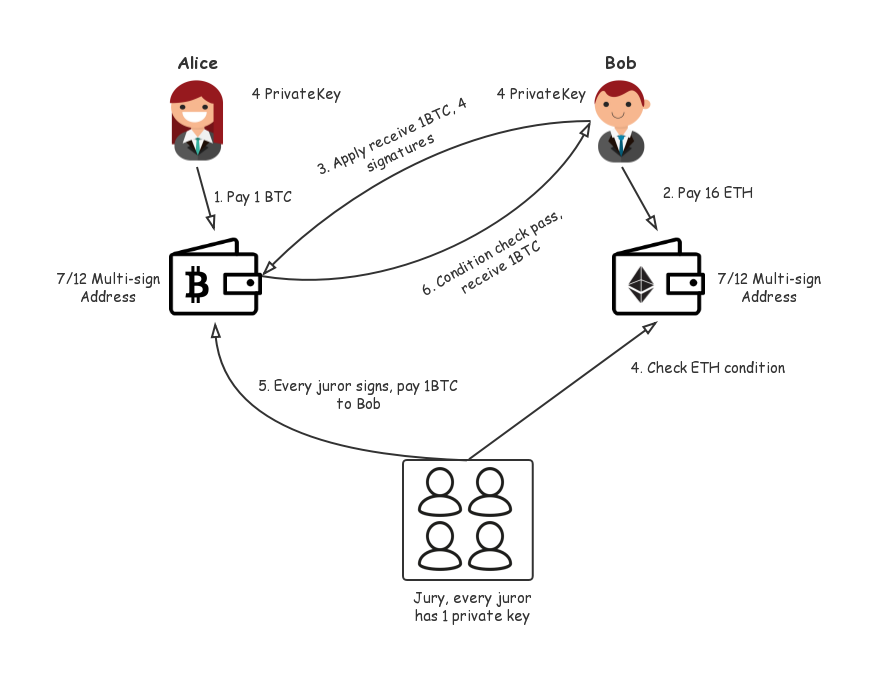
\includegraphics[width=1\textwidth]{./figures/jury.png}
    \centering
    \caption{The normal process of executing the exchange contract (with Jury endorsement) \protect\footnotemark}
    \label{fig:jury}
    \centering
\end{figure}
\footnotetext{Image courtesy of PalletOne yellow paper\cite{palletone}}
\begin{enumerate}
    \item Jury members and two user accounts first executed the proper contract that generated 7/12 multi-signature address for both crypto-currency.
    \item Then both parties transferred a certain amount of exchange currency to corresponding multi-signature address.
    \item Each party will initiate the signature request with their own four private keys to collect the tokens.
    \item Jury verified the validity of both contracts and checked the status of two multi-signature address. If failed, go back to step 2.
    \item After verifying the satisfaction, each juror will sign with the private key and invoke the transactions.
    \item If one party of this transaction failed or timed-out, the Jury will terminate the contract, and there will be a compensation to the other by the one caused the fault.
\end{enumerate}
\begin{figure}[H]
    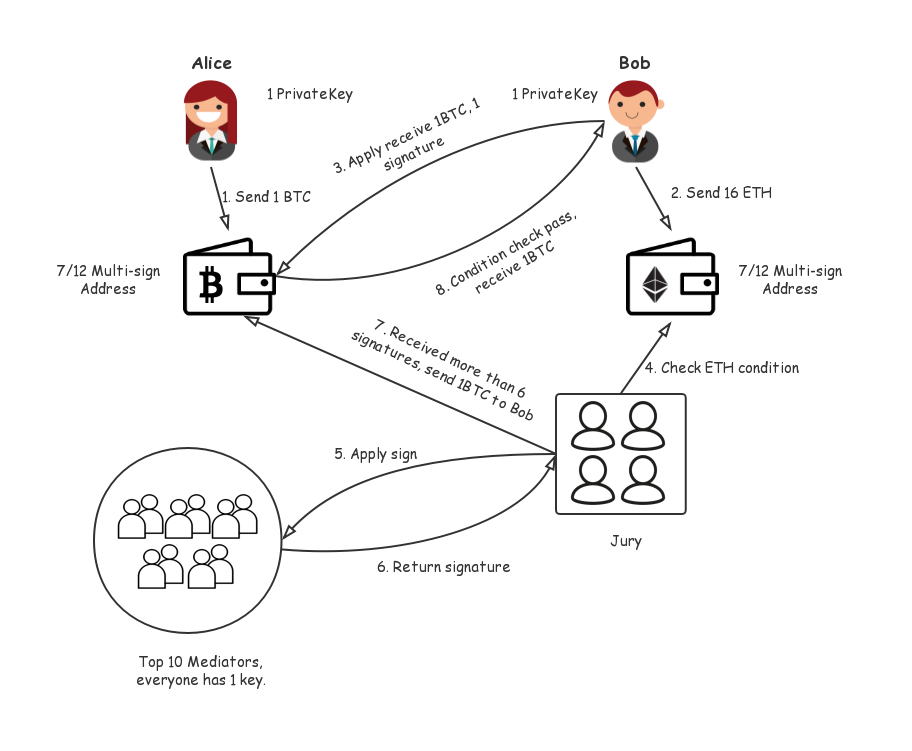
\includegraphics[width=1\textwidth]{./figures/mediator.png}
    \centering
    \caption{The normal process of executing the exchange contract (with Mediator endorsement) \protect\footnotemark}
    \label{fig:mediator}
    \centering
\end{figure}
\footnotetext{Image courtesy of PalletOne yellow paper\cite{palletone}}
\noindent The process of Mediator endorsement during the preparation stage differs from the previous one is, the signed contract will inquire the current votes of the Mediator and select the first ten nodes to form the 7/12 multi-signature address. Also, since the limited number of juror in the Jury endorsement, Mediator mode guarantees the persistence of a multi-signature wallet, so there is additional step for the Jury that has already reached the consensus to send the execution results to Mediators to verify, then the jury leader can broadcast the result once received the majority of Mediators' signature.

\noindent Among the projects I have studied so far, PalletOne has the most ambitious and powerful team with a purely technical project that does not have much community operation.






\section{Summary}
\noindent This Chapter has presented a thorough case study of 14 representative cross-chain projects and classified them into several working schemes. Through the official white paper and other documents, the preceding sections explained the working process and theory of them using diagrams to help the understanding. Including some comments and thoughts towards them. The total work of comparison will be shown as a table in \nameref{app:A}.

%\subsubsection{Liquid}
\noindent Liquid\cite{Liquid} is a sidechain of BTC and a typical representative of the multi-signature notary mechanism. It is designed to meet the BTC fast transfer needs of exchanges, market makers and brokers. Therefore, Liquid uses the multi-sig federation mechanism to confirm the transaction block, which can greatly improve the transaction speed.\\
\noindent Liquid based on Element codebase and uses Strong Federation technology to support 1:1 Bitcoin exchange. The basic process of the transaction is described as Figure \ref{fig:multisig}. The confirmation of this asset transfer requires multi-signature from the majority of notaries.

        \begin{figure}[H]
        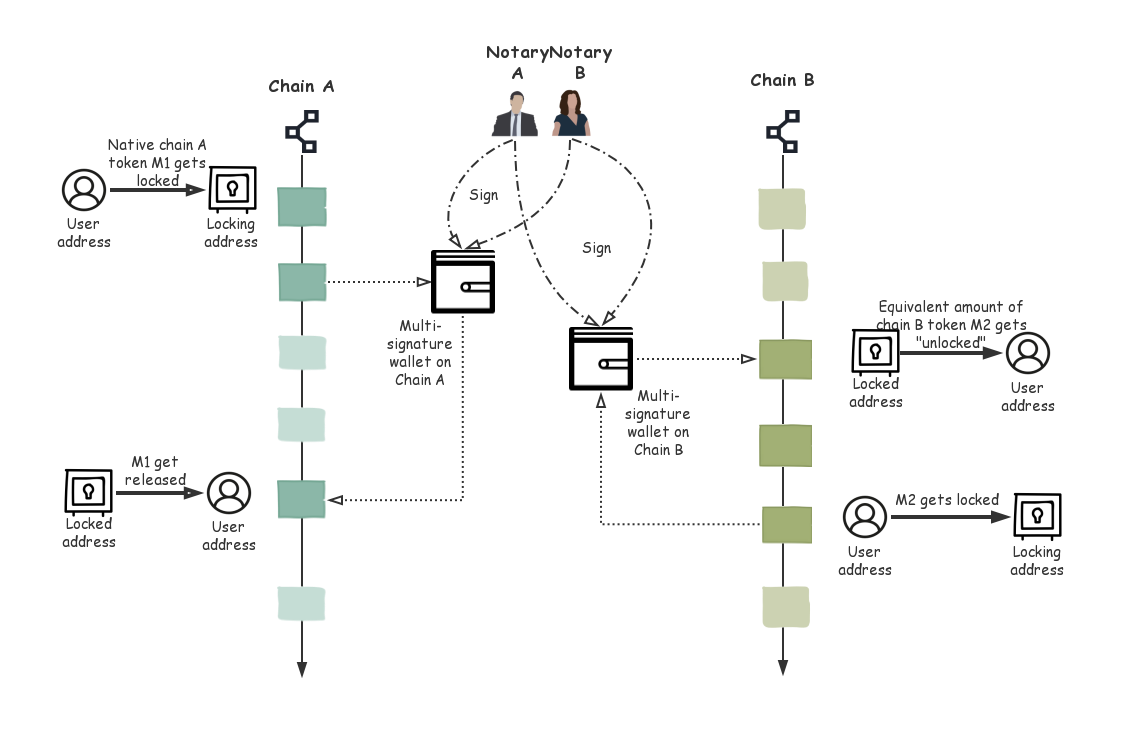
\includegraphics[width=1\textwidth]{./figures/multi_sig.png}
        \centering
        \caption{Multi-signature federation scheme}%\protect\footnotemark}
        \centering
        \label{fig:multisig}
        \end{figure}
        
\noindent In Strong Federation, there are 2 types of node role in the network:
\begin{itemize}
    \item Blocksigners: Signature verification for transactions in the sidechain to achieve block consensus. 
    \item Watchmen: When the asset is transferred from the sidechain to the main chain, it is responsible for signature verification of the transaction on the main chain, indicating that the sidechain asset has indeed been destroyed, and the main chain can unlock the corresponding number of assets.
\end{itemize}

\begin{large}
\textbf{Fusion}
\end{large}\cite{fusion}\\


\noindent Similar to the principle of Wanchain, Fusion's goal is to build a basic platform for the operation of encrypted financial applications based on blockchain technology. On this platform, a variety of tokens can be freely interacted through smart contracts to achieve value interoperability. Support multi-platform cross-chain asset transfer, using a distributed signature notary model for cross-chain transaction processing.\\

\noindent Based on Hierarchical Hybrid Consensus Mechanism(HHCM), Fusion combines the advantages of PoW and PoS consensus mechanism, which balancing the safety, efficiency, and scalability. It is the only cross-chain platform that offers parallel computing, multiple triggering mechanisms, and off-chain data support.\\

        \begin{figure}[H]
        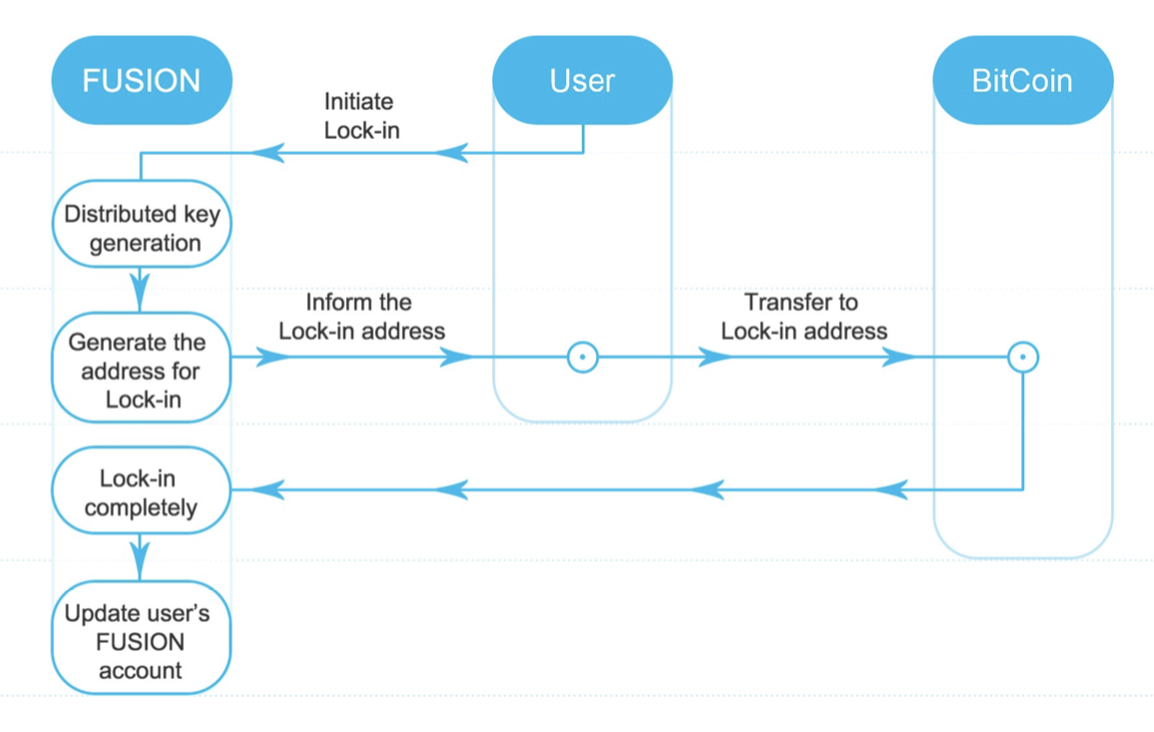
\includegraphics[width=1\textwidth]{./figures/lockin}
        \centering
        \caption{{Fusion Network Architecture, lock-in process}\protect\footnotemark}
        \centering
        \label{fig:lockin}
        
        \end{figure}
\footnotetext{Image courtesy of Fusion white paper\cite{fusion}}
\noindent The realization of cross-chain assets transaction is based on the lock-in\&lock-out process as shown in Figure \ref{fig:lockin}.



\subsubsection{ICON}
\noindent ICON\cite{icon} is committed to building a cross-chain network that connects all types of blockchain systems, enabling DApps to be interconnected across all types of blockchains. The cross-chain transactions primarily handled through notary mechanism. Figure \ref{fig:concept} below shows the overall conceptual model of ICON. With ICON, blockchains are connected around the \textbf{Nexus}, which is a loopchain-based blockchain. The whole system based on loop fault tolerant mechanism which is an enhancement of BFT-based algorithm.  \\


 \begin{figure}[H]
        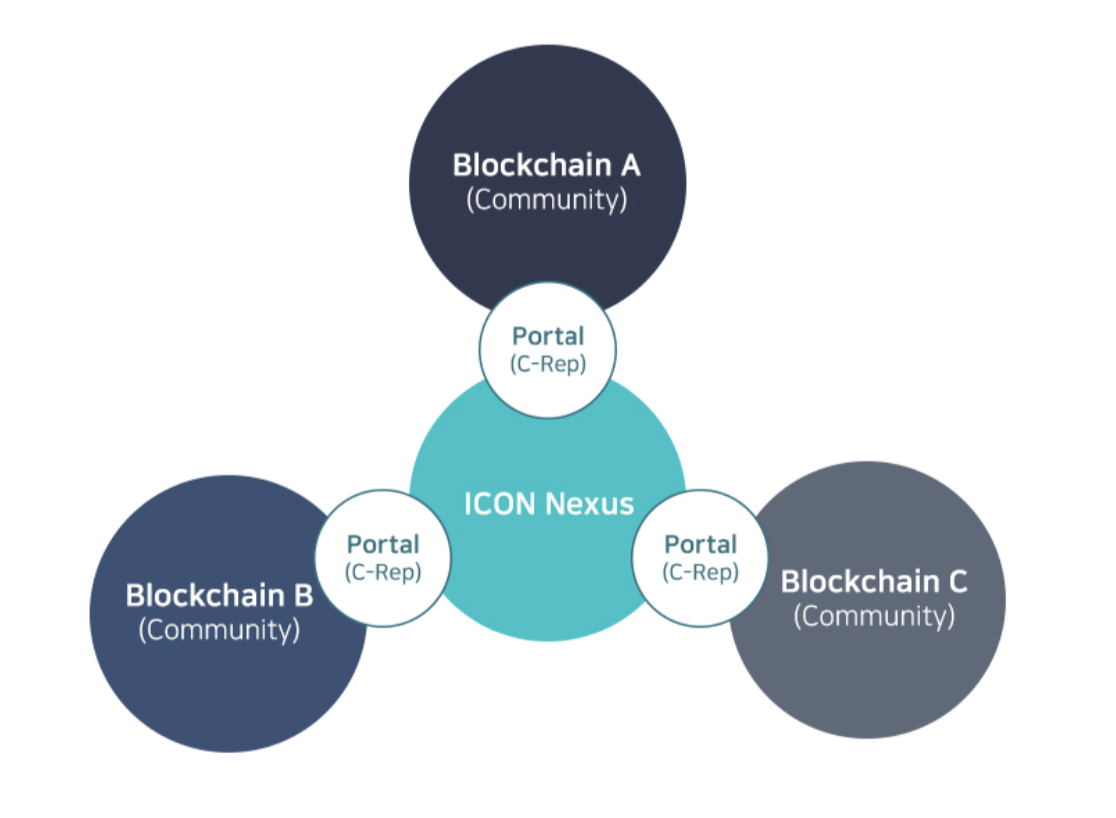
\includegraphics[width=1\textwidth]{./figures/iconconcept.png}
        \centering
        \caption{{Conceptual model of ICON}\protect\footnotemark}
        \centering
        \label{fig:concept}
        
        \end{figure}
\footnotetext{Image courtesy of ICON white paper\cite{icon}, Nexus is a Multi-Channel blockchain comprised of Light Client of respective blockchains. Each blockchain connected to Nexus via a portal.}
        \begin{figure}[H]
        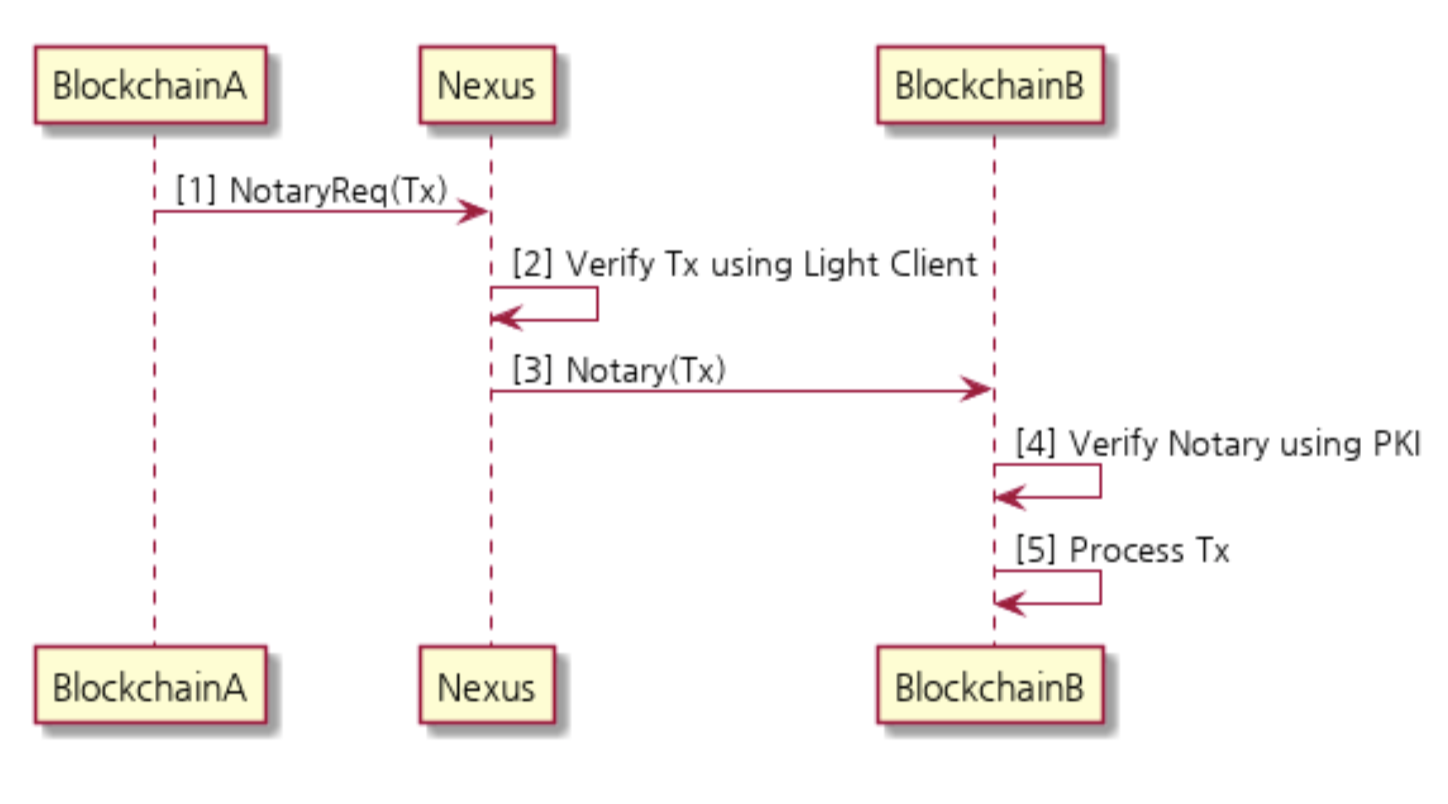
\includegraphics[width=1\textwidth]{./figures/icontrans.png}
        \centering
        \caption{{Assets transaction process through Nexus}\protect\footnotemark}
        \centering
        \label{fig:icon}
        
        \end{figure}
\footnotetext{Image courtesy of ICON white paper\cite{icon}}
\noindent Although rated as one slow progress cross-chain project, ICON still has the ambition to not only connect blockchains together but also aiming at realizing communication between the traditional ledger system and the blockchain world.


\subsubsection{AION}
\noindent Among the Interoperability Alliance\protect\footnotemark
 \footnotetext{Wanchain, ICON and AION form an alliance to overcome the technical difficulties towards cross-chain technology. reference: https://medium.com/helloiconworld/blockchain-interoperability-alliance-icon-x-aion-x-wanchain-8aeaafb3ebdd}
, AION differs from Wanchain and ICON. While the other two projects still focus on the assets and value transactions cross-chain, AION also expanding the business logic and interoperability between chains. Figure\ref{fig:aion} represents a simple multi-tier network architecture based on AION.
        \begin{figure}[H]
        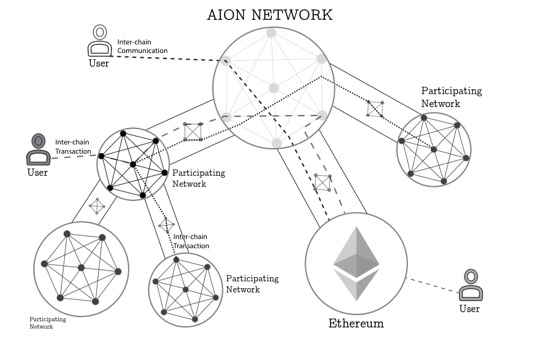
\includegraphics[width=1\textwidth]{./figures/aion.jpg}
        \centering
        \caption{{Multi-tier network structure of AION}\protect\footnotemark}
        \centering
        \label{fig:aion}
        
        \end{figure}
\footnotetext{Image courtesy of AION white paper\cite{aion}}
\noindent AION aims to establish a multi-tier cross-chain platform that supports interoperability of heterogeneous chains. By connecting networks and bridges to blockchain systems, the route of cross-chain transactions is a multi-stage process. \\
\noindent At each stage, the Validators verifies the transaction and agrees on whether the transaction is forwarded or rejected. Bridge validators will use a lightweight BFT-based algorithm to reach consensus. If a transaction is rejected at any time, any state changes due to cross-chain transactions will be revoked, at least in the connected network.\\
\noindent AION has different consensus mechanisms at different product stages, the latest AION 3.0 using mixed DPoS and PoI algorithm.\\
\noindent AION is an emerging project and still in the early stage of development.

\subsubsection{Elastos}
\noindent In order to ease the pressure on the main chain as well as provide better user experience for DApps, Elastos\cite{Elastos} adopted the main chain + sidechain architecture,  main chain only responsible for the circulation of the ELA while the DApps run on the sidechain. \\
\noindent In this scenario, the transfer of the assets between the main chain to sidechain is in a one-to-many relationship. It is feasible that the side chain only saves all the block header information of the main chain. If the main chain needs to save the block header information of all the side chains, it will lead to poor scalability. So Elastos uses asymmetric 2-way peg scheme based on SPV to realize the cross-chain function.\\
\noindent Assets from the main chain to the sidechain, Elastos using SPV proof to prove the transactions, while it secures the transfer using multi-signature notary scheme when transfer from sidechain to the main chain. We can regard this process as a combination of Plasma and Liquid.
.

%\subsubsection{Liquid}
\noindent Liquid\cite{Liquid} is a sidechain of BTC and a typical representative of the multi-signature notary mechanism. It is designed to meet the BTC fast transfer needs of exchanges, market makers and brokers. Therefore, Liquid uses the multi-sig federation mechanism to confirm the transaction block, which can greatly improve the transaction speed.\\
\noindent Liquid based on Element codebase and uses Strong Federation technology to support 1:1 Bitcoin exchange. The basic process of the transaction is described as Figure \ref{fig:multisig}. The confirmation of this asset transfer requires multi-signature from the majority of notaries.

        \begin{figure}[H]
        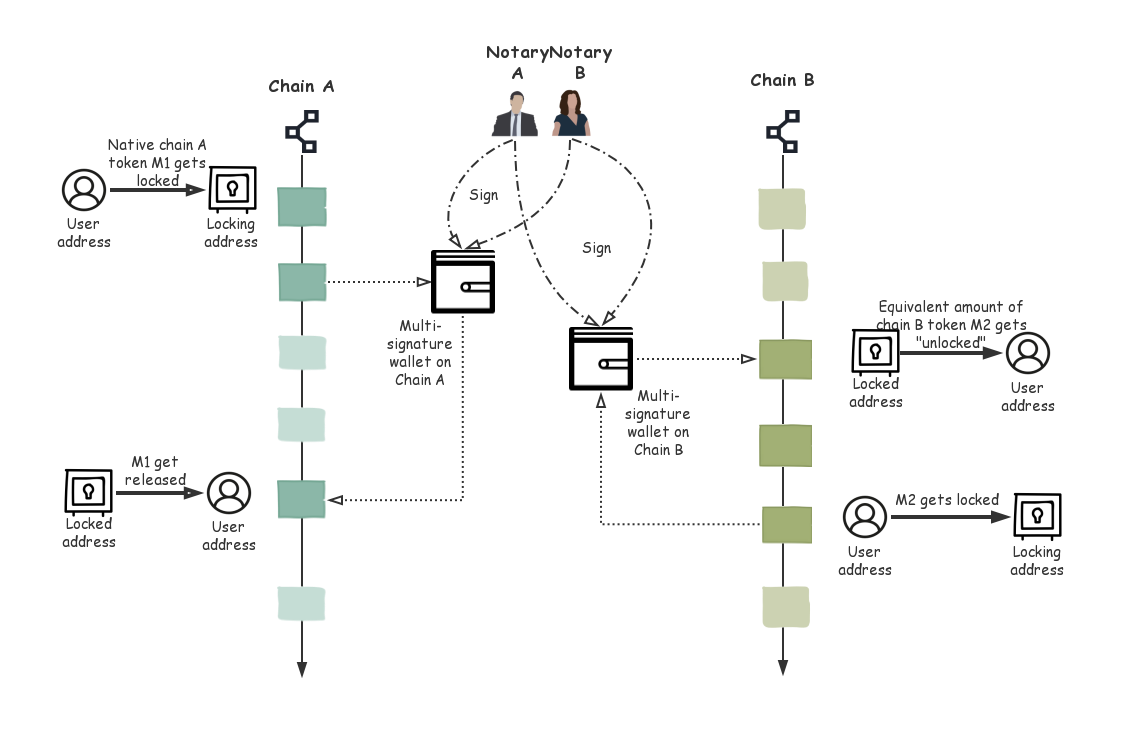
\includegraphics[width=1\textwidth]{./figures/multi_sig.png}
        \centering
        \caption{Multi-signature federation scheme}%\protect\footnotemark}
        \centering
        \label{fig:multisig}
        \end{figure}
        
\noindent In Strong Federation, there are 2 types of node role in the network:
\begin{itemize}
    \item Blocksigners: Signature verification for transactions in the sidechain to achieve block consensus. 
    \item Watchmen: When the asset is transferred from the sidechain to the main chain, it is responsible for signature verification of the transaction on the main chain, indicating that the sidechain asset has indeed been destroyed, and the main chain can unlock the corresponding number of assets.
\end{itemize}

\begin{large}
\textbf{Fusion}
\end{large}\cite{fusion}\\


\noindent Similar to the principle of Wanchain, Fusion's goal is to build a basic platform for the operation of encrypted financial applications based on blockchain technology. On this platform, a variety of tokens can be freely interacted through smart contracts to achieve value interoperability. Support multi-platform cross-chain asset transfer, using a distributed signature notary model for cross-chain transaction processing.\\

\noindent Based on Hierarchical Hybrid Consensus Mechanism(HHCM), Fusion combines the advantages of PoW and PoS consensus mechanism, which balancing the safety, efficiency, and scalability. It is the only cross-chain platform that offers parallel computing, multiple triggering mechanisms, and off-chain data support.\\

        \begin{figure}[H]
        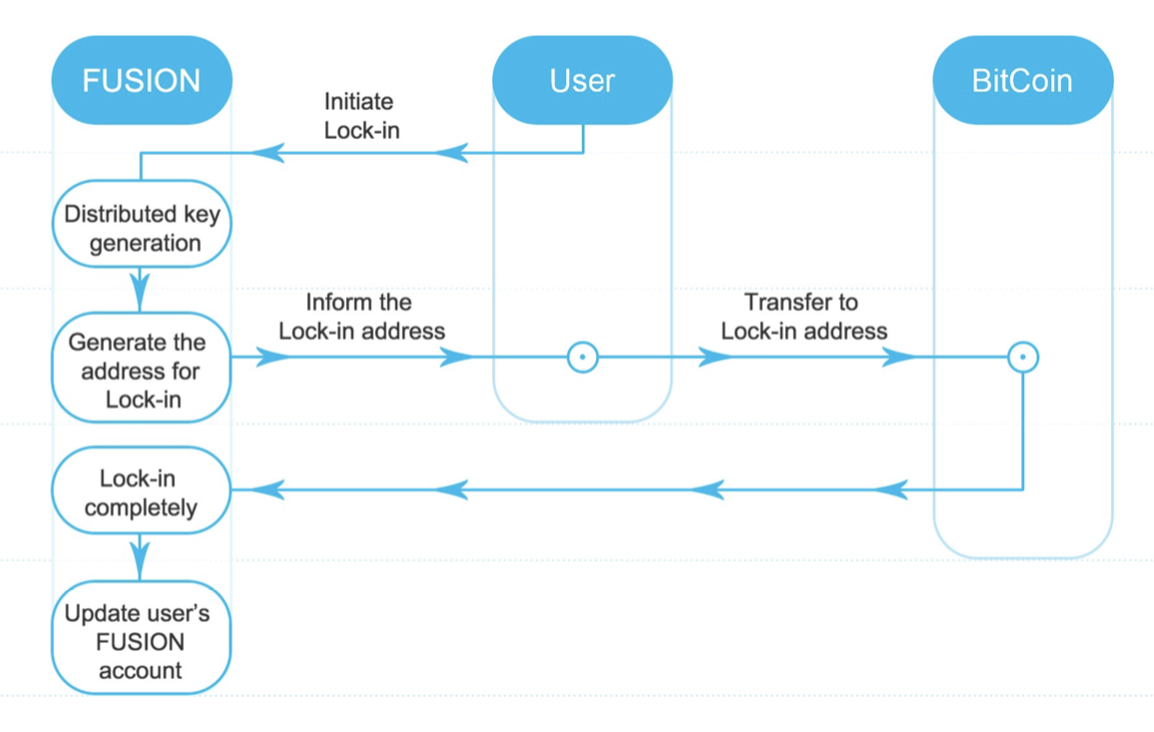
\includegraphics[width=1\textwidth]{./figures/lockin}
        \centering
        \caption{{Fusion Network Architecture, lock-in process}\protect\footnotemark}
        \centering
        \label{fig:lockin}
        
        \end{figure}
\footnotetext{Image courtesy of Fusion white paper\cite{fusion}}
\noindent The realization of cross-chain assets transaction is based on the lock-in\&lock-out process as shown in Figure \ref{fig:lockin}.



\subsubsection{ICON}
\noindent ICON\cite{icon} is committed to building a cross-chain network that connects all types of blockchain systems, enabling DApps to be interconnected across all types of blockchains. The cross-chain transactions primarily handled through notary mechanism. Figure \ref{fig:concept} below shows the overall conceptual model of ICON. With ICON, blockchains are connected around the \textbf{Nexus}, which is a loopchain-based blockchain. The whole system based on loop fault tolerant mechanism which is an enhancement of BFT-based algorithm.  \\


 \begin{figure}[H]
        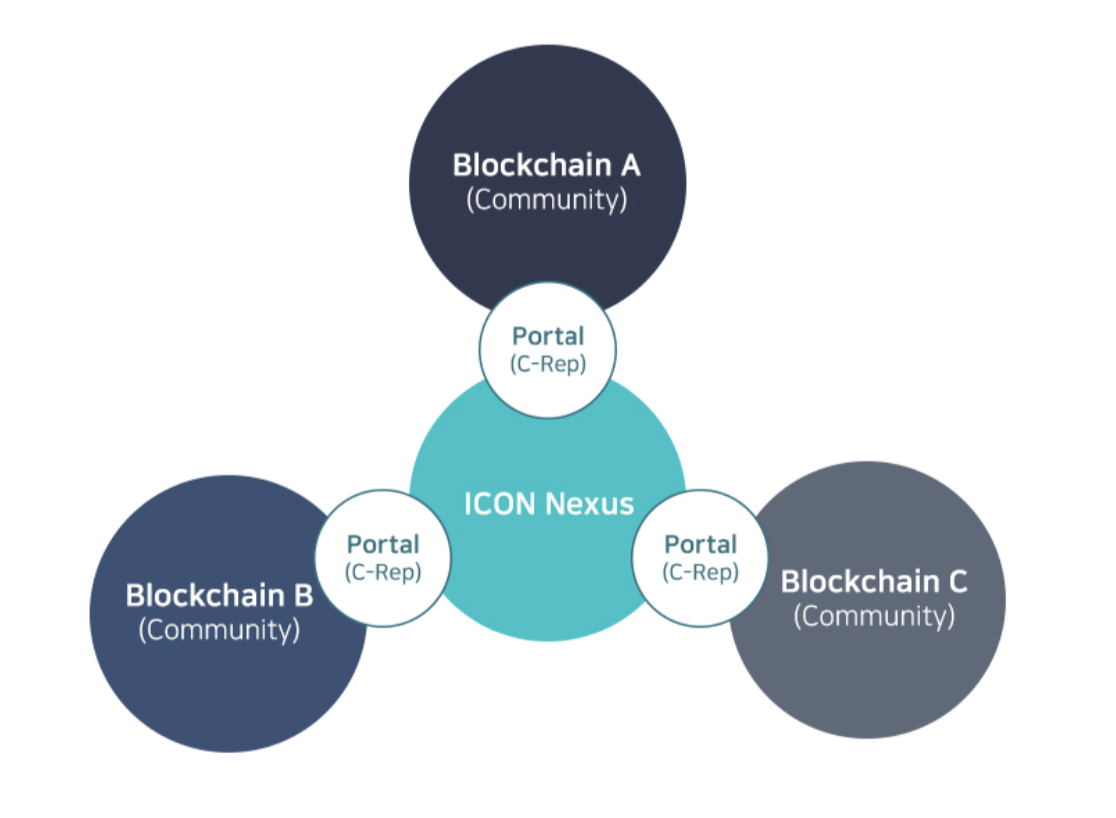
\includegraphics[width=1\textwidth]{./figures/iconconcept.png}
        \centering
        \caption{{Conceptual model of ICON}\protect\footnotemark}
        \centering
        \label{fig:concept}
        
        \end{figure}
\footnotetext{Image courtesy of ICON white paper\cite{icon}, Nexus is a Multi-Channel blockchain comprised of Light Client of respective blockchains. Each blockchain connected to Nexus via a portal.}
        \begin{figure}[H]
        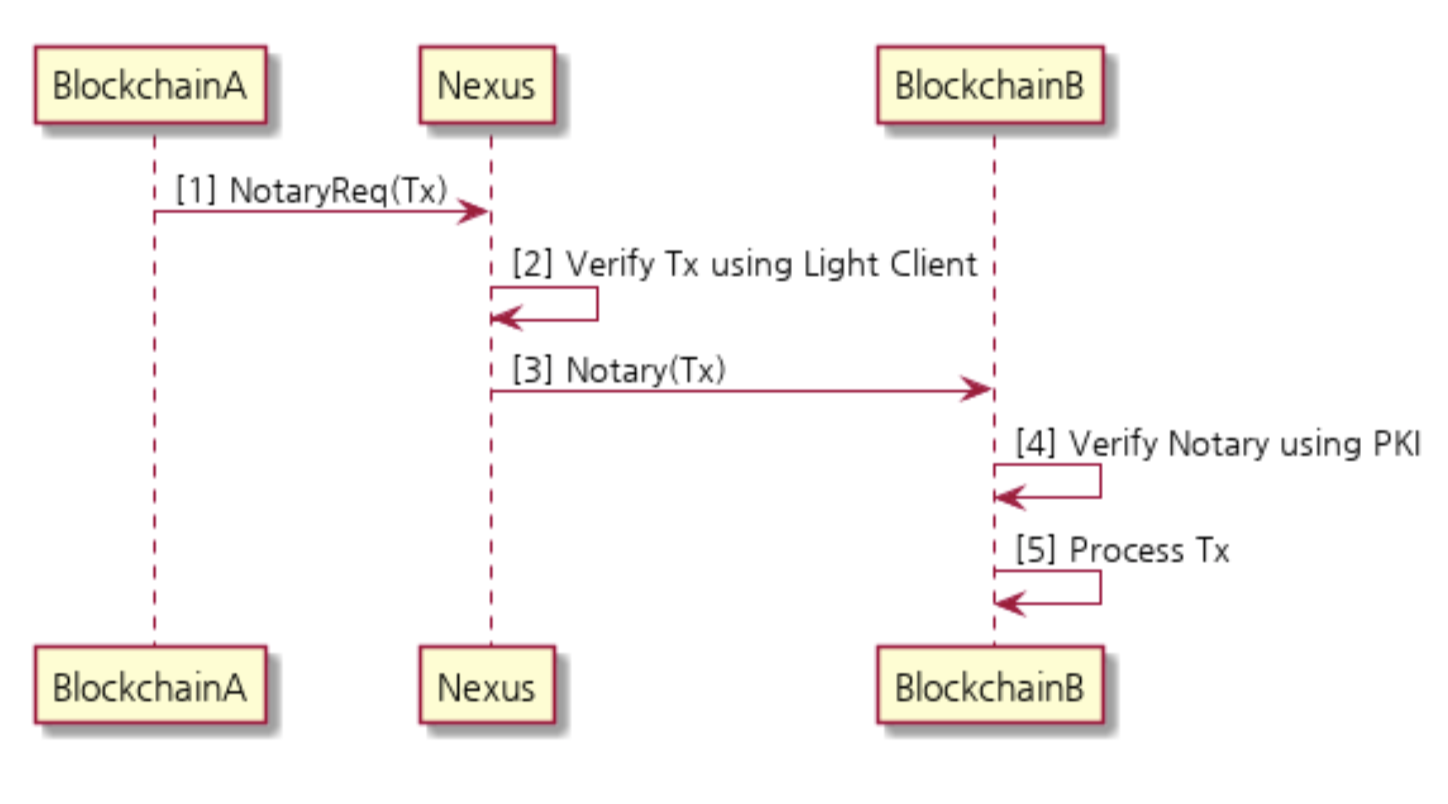
\includegraphics[width=1\textwidth]{./figures/icontrans.png}
        \centering
        \caption{{Assets transaction process through Nexus}\protect\footnotemark}
        \centering
        \label{fig:icon}
        
        \end{figure}
\footnotetext{Image courtesy of ICON white paper\cite{icon}}
\noindent Although rated as one slow progress cross-chain project, ICON still has the ambition to not only connect blockchains together but also aiming at realizing communication between the traditional ledger system and the blockchain world.


\subsubsection{AION}
\noindent Among the Interoperability Alliance\protect\footnotemark
 \footnotetext{Wanchain, ICON and AION form an alliance to overcome the technical difficulties towards cross-chain technology. reference: https://medium.com/helloiconworld/blockchain-interoperability-alliance-icon-x-aion-x-wanchain-8aeaafb3ebdd}
, AION differs from Wanchain and ICON. While the other two projects still focus on the assets and value transactions cross-chain, AION also expanding the business logic and interoperability between chains. Figure\ref{fig:aion} represents a simple multi-tier network architecture based on AION.
        \begin{figure}[H]
        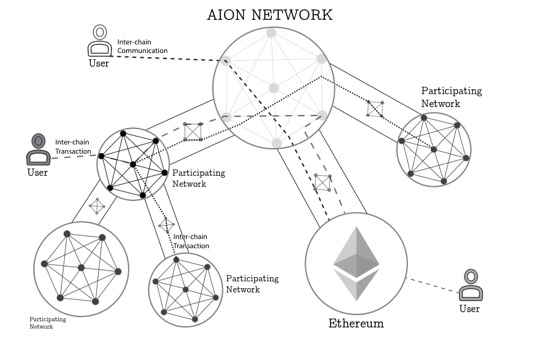
\includegraphics[width=1\textwidth]{./figures/aion.jpg}
        \centering
        \caption{{Multi-tier network structure of AION}\protect\footnotemark}
        \centering
        \label{fig:aion}
        
        \end{figure}
\footnotetext{Image courtesy of AION white paper\cite{aion}}
\noindent AION aims to establish a multi-tier cross-chain platform that supports interoperability of heterogeneous chains. By connecting networks and bridges to blockchain systems, the route of cross-chain transactions is a multi-stage process. \\
\noindent At each stage, the Validators verifies the transaction and agrees on whether the transaction is forwarded or rejected. Bridge validators will use a lightweight BFT-based algorithm to reach consensus. If a transaction is rejected at any time, any state changes due to cross-chain transactions will be revoked, at least in the connected network.\\
\noindent AION has different consensus mechanisms at different product stages, the latest AION 3.0 using mixed DPoS and PoI algorithm.\\
\noindent AION is an emerging project and still in the early stage of development.

\subsubsection{Elastos}
\noindent In order to ease the pressure on the main chain as well as provide better user experience for DApps, Elastos\cite{Elastos} adopted the main chain + sidechain architecture,  main chain only responsible for the circulation of the ELA while the DApps run on the sidechain. \\
\noindent In this scenario, the transfer of the assets between the main chain to sidechain is in a one-to-many relationship. It is feasible that the side chain only saves all the block header information of the main chain. If the main chain needs to save the block header information of all the side chains, it will lead to poor scalability. So Elastos uses asymmetric 2-way peg scheme based on SPV to realize the cross-chain function.\\
\noindent Assets from the main chain to the sidechain, Elastos using SPV proof to prove the transactions, while it secures the transfer using multi-signature notary scheme when transfer from sidechain to the main chain. We can regard this process as a combination of Plasma and Liquid.
